\documentclass[]{article}
\usepackage{lmodern}
\usepackage{amssymb,amsmath}
\usepackage{ifxetex,ifluatex}
\usepackage{fixltx2e} % provides \textsubscript
\ifnum 0\ifxetex 1\fi\ifluatex 1\fi=0 % if pdftex
  \usepackage[T1]{fontenc}
  \usepackage[utf8]{inputenc}
\else % if luatex or xelatex
  \ifxetex
    \usepackage{mathspec}
  \else
    \usepackage{fontspec}
  \fi
  \defaultfontfeatures{Ligatures=TeX,Scale=MatchLowercase}
\fi
% use upquote if available, for straight quotes in verbatim environments
\IfFileExists{upquote.sty}{\usepackage{upquote}}{}
% use microtype if available
\IfFileExists{microtype.sty}{%
\usepackage{microtype}
\UseMicrotypeSet[protrusion]{basicmath} % disable protrusion for tt fonts
}{}
\usepackage[margin=1in]{geometry}
\usepackage{hyperref}
\hypersetup{unicode=true,
            pdftitle={NZ Electricity Generation Trends 1998-2017},
            pdfauthor={Ben Anderson (b.anderson@soton.ac.uk @dataknut)},
            pdfborder={0 0 0},
            breaklinks=true}
\urlstyle{same}  % don't use monospace font for urls
\usepackage{color}
\usepackage{fancyvrb}
\newcommand{\VerbBar}{|}
\newcommand{\VERB}{\Verb[commandchars=\\\{\}]}
\DefineVerbatimEnvironment{Highlighting}{Verbatim}{commandchars=\\\{\}}
% Add ',fontsize=\small' for more characters per line
\usepackage{framed}
\definecolor{shadecolor}{RGB}{248,248,248}
\newenvironment{Shaded}{\begin{snugshade}}{\end{snugshade}}
\newcommand{\KeywordTok}[1]{\textcolor[rgb]{0.13,0.29,0.53}{\textbf{#1}}}
\newcommand{\DataTypeTok}[1]{\textcolor[rgb]{0.13,0.29,0.53}{#1}}
\newcommand{\DecValTok}[1]{\textcolor[rgb]{0.00,0.00,0.81}{#1}}
\newcommand{\BaseNTok}[1]{\textcolor[rgb]{0.00,0.00,0.81}{#1}}
\newcommand{\FloatTok}[1]{\textcolor[rgb]{0.00,0.00,0.81}{#1}}
\newcommand{\ConstantTok}[1]{\textcolor[rgb]{0.00,0.00,0.00}{#1}}
\newcommand{\CharTok}[1]{\textcolor[rgb]{0.31,0.60,0.02}{#1}}
\newcommand{\SpecialCharTok}[1]{\textcolor[rgb]{0.00,0.00,0.00}{#1}}
\newcommand{\StringTok}[1]{\textcolor[rgb]{0.31,0.60,0.02}{#1}}
\newcommand{\VerbatimStringTok}[1]{\textcolor[rgb]{0.31,0.60,0.02}{#1}}
\newcommand{\SpecialStringTok}[1]{\textcolor[rgb]{0.31,0.60,0.02}{#1}}
\newcommand{\ImportTok}[1]{#1}
\newcommand{\CommentTok}[1]{\textcolor[rgb]{0.56,0.35,0.01}{\textit{#1}}}
\newcommand{\DocumentationTok}[1]{\textcolor[rgb]{0.56,0.35,0.01}{\textbf{\textit{#1}}}}
\newcommand{\AnnotationTok}[1]{\textcolor[rgb]{0.56,0.35,0.01}{\textbf{\textit{#1}}}}
\newcommand{\CommentVarTok}[1]{\textcolor[rgb]{0.56,0.35,0.01}{\textbf{\textit{#1}}}}
\newcommand{\OtherTok}[1]{\textcolor[rgb]{0.56,0.35,0.01}{#1}}
\newcommand{\FunctionTok}[1]{\textcolor[rgb]{0.00,0.00,0.00}{#1}}
\newcommand{\VariableTok}[1]{\textcolor[rgb]{0.00,0.00,0.00}{#1}}
\newcommand{\ControlFlowTok}[1]{\textcolor[rgb]{0.13,0.29,0.53}{\textbf{#1}}}
\newcommand{\OperatorTok}[1]{\textcolor[rgb]{0.81,0.36,0.00}{\textbf{#1}}}
\newcommand{\BuiltInTok}[1]{#1}
\newcommand{\ExtensionTok}[1]{#1}
\newcommand{\PreprocessorTok}[1]{\textcolor[rgb]{0.56,0.35,0.01}{\textit{#1}}}
\newcommand{\AttributeTok}[1]{\textcolor[rgb]{0.77,0.63,0.00}{#1}}
\newcommand{\RegionMarkerTok}[1]{#1}
\newcommand{\InformationTok}[1]{\textcolor[rgb]{0.56,0.35,0.01}{\textbf{\textit{#1}}}}
\newcommand{\WarningTok}[1]{\textcolor[rgb]{0.56,0.35,0.01}{\textbf{\textit{#1}}}}
\newcommand{\AlertTok}[1]{\textcolor[rgb]{0.94,0.16,0.16}{#1}}
\newcommand{\ErrorTok}[1]{\textcolor[rgb]{0.64,0.00,0.00}{\textbf{#1}}}
\newcommand{\NormalTok}[1]{#1}
\usepackage{longtable,booktabs}
\usepackage{graphicx,grffile}
\makeatletter
\def\maxwidth{\ifdim\Gin@nat@width>\linewidth\linewidth\else\Gin@nat@width\fi}
\def\maxheight{\ifdim\Gin@nat@height>\textheight\textheight\else\Gin@nat@height\fi}
\makeatother
% Scale images if necessary, so that they will not overflow the page
% margins by default, and it is still possible to overwrite the defaults
% using explicit options in \includegraphics[width, height, ...]{}
\setkeys{Gin}{width=\maxwidth,height=\maxheight,keepaspectratio}
\IfFileExists{parskip.sty}{%
\usepackage{parskip}
}{% else
\setlength{\parindent}{0pt}
\setlength{\parskip}{6pt plus 2pt minus 1pt}
}
\setlength{\emergencystretch}{3em}  % prevent overfull lines
\providecommand{\tightlist}{%
  \setlength{\itemsep}{0pt}\setlength{\parskip}{0pt}}
\setcounter{secnumdepth}{5}
% Redefines (sub)paragraphs to behave more like sections
\ifx\paragraph\undefined\else
\let\oldparagraph\paragraph
\renewcommand{\paragraph}[1]{\oldparagraph{#1}\mbox{}}
\fi
\ifx\subparagraph\undefined\else
\let\oldsubparagraph\subparagraph
\renewcommand{\subparagraph}[1]{\oldsubparagraph{#1}\mbox{}}
\fi

%%% Use protect on footnotes to avoid problems with footnotes in titles
\let\rmarkdownfootnote\footnote%
\def\footnote{\protect\rmarkdownfootnote}

%%% Change title format to be more compact
\usepackage{titling}

% Create subtitle command for use in maketitle
\newcommand{\subtitle}[1]{
  \posttitle{
    \begin{center}\large#1\end{center}
    }
}

\setlength{\droptitle}{-2em}

  \title{NZ Electricity Generation Trends 1998-2017}
    \pretitle{\vspace{\droptitle}\centering\huge}
  \posttitle{\par}
    \author{Ben Anderson
(\href{mailto:b.anderson@soton.ac.uk}{\nolinkurl{b.anderson@soton.ac.uk}}
\texttt{@dataknut})}
    \preauthor{\centering\large\emph}
  \postauthor{\par}
      \predate{\centering\large\emph}
  \postdate{\par}
    \date{Last run at: 2018-06-28 09:37:07}


\usepackage{amsthm}
\newtheorem{theorem}{Theorem}[section]
\newtheorem{lemma}{Lemma}[section]
\theoremstyle{definition}
\newtheorem{definition}{Definition}[section]
\newtheorem{corollary}{Corollary}[section]
\newtheorem{proposition}{Proposition}[section]
\theoremstyle{definition}
\newtheorem{example}{Example}[section]
\theoremstyle{definition}
\newtheorem{exercise}{Exercise}[section]
\theoremstyle{remark}
\newtheorem*{remark}{Remark}
\newtheorem*{solution}{Solution}
\begin{document}
\maketitle

{
\setcounter{tocdepth}{2}
\tableofcontents
}
\newpage

\section{Citation}\label{citation}

If you wish to use any of the material from this report please cite as:

\begin{itemize}
\tightlist
\item
  Anderson, B. (2018) \emph{NZ Electricity Generation Trends 1998-2017},
  \href{http://www.otago.ac.nz/centre-sustainability/}{Centre for
  Sustainability}, University of Otago: Dunedin.
\end{itemize}

This work is (c) 2018 the University of Southampton.

\newpage

\section{About}\label{about}

\subsection{Circulation}\label{circulation}

Report circulation:

\begin{itemize}
\tightlist
\item
  Restricted to:
  \href{https://www.otago.ac.nz/centre-sustainability/research/energy/otago050285.html}{NZ
  GREEN Grid} project partners and contractors.
\end{itemize}

\subsection{Purpose}\label{purpose}

This report is intended to:

\begin{itemize}
\tightlist
\item
  load and test NZ electricity generation data from
  \url{https://www.emi.ea.govt.nz/Wholesale/Datasets/Generation/Generation_MD/}
  from 1998 to 2017.
\end{itemize}

\subsection{Requirements:}\label{requirements}

\begin{itemize}
\tightlist
\item
  pre-downloaded NZ wholesale generation datasets
\end{itemize}

\subsection{History}\label{history}

Generally tracked via our git.soton
\href{https://git.soton.ac.uk/ba1e12/nzGREENGrid}{repo}:

\begin{itemize}
\tightlist
\item
  \href{https://git.soton.ac.uk/ba1e12/nzGREENGrid/commits/master}{history}
\item
  \href{https://git.soton.ac.uk/ba1e12/nzGREENGrid/issues}{issues}
\end{itemize}

Specific history of this code:

\begin{itemize}
\tightlist
\item
  \url{https://git.soton.ac.uk/ba1e12/nzGREENGrid/commits/master/analysis/generation/nzGenerationHistory.Rmd}
\end{itemize}

\subsection{Support}\label{support}

This work was supported by:

\begin{itemize}
\tightlist
\item
  The \href{https://www.otago.ac.nz/}{University of Otago};
\item
  The \href{https://www.southampton.ac.uk/}{University of Southampton};
\item
  The New Zealand \href{http://www.mbie.govt.nz/}{Ministry of Business,
  Innovation and Employment (MBIE)} through the
  \href{https://www.otago.ac.nz/centre-sustainability/research/energy/otago050285.html}{NZ
  GREEN Grid} project;
\item
  \href{http://www.energy.soton.ac.uk/tag/spatialec/}{SPATIALEC} - a
  \href{http://ec.europa.eu/research/mariecurieactions/about-msca/actions/if/index_en.htm}{Marie
  Skłodowska-Curie Global Fellowship} based at the University of Otago's
  \href{http://www.otago.ac.nz/centre-sustainability/staff/otago673896.html}{Centre
  for Sustainability} (2017-2019) \& the University of Southampton's
  Sustainable Energy Research Group (2019-202).
\end{itemize}

We do not `support' the code but if you have a problem check the
\href{https://git.soton.ac.uk/ba1e12/nzGREENGrid/issues}{issues} on our
\href{https://git.soton.ac.uk/ba1e12/nzGREENGrid}{repo} and if it
doesn't already exist, open one. We might be able to fix it :-)

\section{Introduction}\label{introduction}

Inspired by Steffel
(\href{https://www.sciencedirect.com/science/article/pii/S0301421516307017}{2018})
which analyses trends in the type and timing of generation in the UK
over the same time period. Intended to build on Kahn et al's 2018 CO2
\href{https://www.sciencedirect.com/science/article/pii/S0959652618306474?via\%3Dihub}{intensity
of peak demand} paper - how have thngs changed over time?

Uses
\url{https://www.emi.ea.govt.nz/Wholesale/Datasets/Generation/Generation_MD/}
from 1998 to 2017. Note that this does not appear to include Solar (too
low or in a seperate data set?) nor does it appear to include
domestic/small-scale generation? It is possible that these are to be
found in
\url{https://www.emi.ea.govt.nz/Wholesale/Datasets/Metered_data/Embedded_generation}
and should be combined with this data?

Data is kWh - so energy not power.

\section{~Load data}\label{load-data}

Load the generation data from files stored in:

\begin{itemize}
\tightlist
\item
  /Volumes/hum-csafe/Research Projects/GREEN Grid/\_RAW
  DATA/EA\_Generation\_Data/
\end{itemize}

These have been
\href{https://git.soton.ac.uk/ba1e12/nzGREENGrid/tree/master/dataProcessing/ea}{pre-downloaded
and cleaned} but could be pulled on the fly to be refreshed for other
dates\ldots{}

\begin{verbatim}
## Warning in `[.data.table`(filesToDateDT, , `:=`(c("year", "month",
## "stub"), : Supplied 3 columns to be assigned a list (length 5) of values (2
## unused)
\end{verbatim}

\begin{verbatim}
## [1] "Files loaded"
\end{verbatim}

\begin{verbatim}
## [1] "Loaded 352,250 rows of data"
\end{verbatim}

\begin{verbatim}
## sampleGenDT 
## 
##  14  Variables      352250  Observations
## ---------------------------------------------------------------------------
## Site_Code 
##        n  missing distinct 
##   352250        0       69 
## 
## lowest : ANI ARA ARG ARI ATI, highest: WPA WPI WRK WTK WWD
## ---------------------------------------------------------------------------
## POC_Code 
##        n  missing distinct 
##   352250        0       68 
## 
## lowest : ARA2201 ARG1101 ARI1101 ARI1102 ASB0661
## highest: WRK0331 WRK2201 WTK0111 WWD1102 WWD1103
## ---------------------------------------------------------------------------
## Nwk_Code 
##        n  missing distinct 
##   352250        0       27 
## 
## lowest : ALNT BOPD CHHE CTCT EASH, highest: TRPG TRUS TUAR WAIK WATA
## ---------------------------------------------------------------------------
## Gen_Code 
##        n  missing distinct 
##   352250        0       68 
## 
## lowest : aniwhenua     arapuni       aratiatia     argyle_wairau atiamuri     
## highest: whakamaru     whareroa      wheao_flaxy   whirinaki     white_hill   
## ---------------------------------------------------------------------------
## Fuel_Code 
##        n  missing distinct 
##   352250        0        8 
##                                                                           
## Value         Coal  Diesel     Gas Gas&Oil     Geo   Hydro    Wind    Wood
## Frequency     6100    6100   44300    6100   42700  213500   27350    6100
## Proportion   0.017   0.017   0.126   0.017   0.121   0.606   0.078   0.017
## ---------------------------------------------------------------------------
## Tech_Code 
##        n  missing distinct 
##   352250        0        5 
##                                              
## Value       Cogen    Geo  Hydro  Thrml   Wind
## Frequency   27500  42700 213500  41200  27350
## Proportion  0.078  0.121  0.606  0.117  0.078
## ---------------------------------------------------------------------------
## Trading_date 
##        n  missing distinct 
##   352250        0      122 
## 
## lowest : 1998-06-01 1998-06-02 1998-06-03 1998-06-04 1998-06-05
## highest: 2017-12-27 2017-12-28 2017-12-29 2017-12-30 2017-12-31
## ---------------------------------------------------------------------------
## Time_Period 
##        n  missing distinct 
##   352250        0       50 
## 
## lowest : TP1  TP10 TP11 TP12 TP13, highest: TP50 TP6  TP7  TP8  TP9 
## ---------------------------------------------------------------------------
## kWh 
##        n  missing distinct     Info     Mean      Gmd      .05      .10 
##   338160    14090   116836    0.997    37186    45162        0        0 
##      .25      .50      .75      .90      .95 
##     6563    19715    48640    82910   150714 
## 
## lowest : 0.0000e+00 4.5000e-03 8.7000e-03 1.0000e-02 1.0200e-02
## highest: 4.9213e+05 4.9239e+05 4.9246e+05 4.9266e+05 4.9302e+05
## ---------------------------------------------------------------------------
## rTime [secs] 
##        n  missing distinct 
##   338160    14090       48 
## 
## lowest : 00:15:00 00:45:00 01:15:00 01:45:00 02:15:00
## highest: 21:45:00 22:15:00 22:45:00 23:15:00 23:45:00
## ---------------------------------------------------------------------------
## rDate 
##        n  missing distinct 
##   352250        0      122 
## 
## lowest : 1998-06-01 1998-06-02 1998-06-03 1998-06-04 1998-06-05
## highest: 2017-12-27 2017-12-28 2017-12-29 2017-12-30 2017-12-31
## ---------------------------------------------------------------------------
## rDateTime 
##                   n             missing            distinct 
##              338160               14090                5856 
##                Info                Mean                 Gmd 
##                   1 2010-03-23 19:23:45 1979-03-18 16:00:26 
##                 .05                 .10                 .25 
## 1998-06-09 00:15:00 1998-06-17 00:15:00 1998-12-10 09:15:00 
##                 .50                 .75                 .90 
## 2017-06-11 15:45:00 2017-12-06 19:15:00 2017-12-21 22:15:00 
##                 .95 
## 2017-12-26 23:15:00 
##                                                                       
## Value      8.950e+08 9.000e+08 9.100e+08 9.150e+08 1.495e+09 1.500e+09
## Frequency      20548     42812       752     69184     47600     53200
## Proportion     0.061     0.127     0.002     0.205     0.141     0.157
##                               
## Value      1.510e+09 1.515e+09
## Frequency      16100     87964
## Proportion     0.048     0.260
## ---------------------------------------------------------------------------
## month 
##        n  missing distinct     Info     Mean      Gmd 
##   352250        0        2    0.749    9.087    2.997 
##                         
## Value           6     12
## Frequency  171000 181250
## Proportion  0.485  0.515
## ---------------------------------------------------------------------------
## year 
##        n  missing distinct     Info     Mean      Gmd 
##   352250        0        2    0.716     2010    9.075 
##                         
## Value        1998   2017
## Frequency  138850 213400
## Proportion  0.394  0.606
## ---------------------------------------------------------------------------
\end{verbatim}

Table \ref{tab:finalSummary} sumarises the data. Notice that there are
missing (NA) values in the kWh column. These are caused by periods 49
and 50:

\begin{quote}
``The data is presented by trading period, TP1, TP2, \ldots{} TP48.
Trading period 1 starts at midnight, trading period 2 starts at 12:30am,
trading period 3 starts at 1:00am, etc. Users of this data should be
aware of daylight saving in New Zealand. On the day daylight saving
commences there are only 46 trading periods and on the day it ends,
there are 50.''
(\url{https://www.emi.ea.govt.nz/Wholesale/Datasets/Generation/Generation_MD/})
\end{quote}

So on 2 days of the year TP47 \& TP48 do not exist and on the following
days they are back and we also have TP49 \& TP50. There are only two
things in life worse than death \& taxes: daylight saving time and
time-zones.

Daylight saving begins/ends in October and March so we carefully avoid
this problem in this section by using June and December. However these
TP are still present as labels in the Time\_Period variable and so give
NA kWh in the data as the following table (Table \ref{tab:exploreNA})
and plot (Figure \ref{fig:exploreNA}) of NA observations (only) by Fuel
Type and month show.

\begin{table}

\caption{\label{tab:exploreNA}Mean kWh by Time Period}
\centering
\begin{tabular}[t]{l|r}
\hline
Time\_Period & mean\\
\hline
TP1 & 32193.95\\
\hline
TP10 & 28197.44\\
\hline
TP11 & 29102.29\\
\hline
TP12 & 30355.92\\
\hline
TP13 & 32589.18\\
\hline
TP14 & 35307.47\\
\hline
TP15 & 38153.58\\
\hline
TP16 & 40611.99\\
\hline
TP17 & 41846.03\\
\hline
TP18 & 42344.12\\
\hline
TP19 & 42572.59\\
\hline
TP2 & 31058.35\\
\hline
TP20 & 42364.31\\
\hline
TP21 & 41953.33\\
\hline
TP22 & 41580.21\\
\hline
TP23 & 41157.60\\
\hline
TP24 & 40811.56\\
\hline
TP25 & 40331.06\\
\hline
TP26 & 39886.99\\
\hline
TP27 & 39653.17\\
\hline
TP28 & 39227.72\\
\hline
TP29 & 38878.22\\
\hline
TP3 & 30111.71\\
\hline
TP30 & 38668.61\\
\hline
TP31 & 38707.44\\
\hline
TP32 & 39144.56\\
\hline
TP33 & 39847.08\\
\hline
TP34 & 41145.00\\
\hline
TP35 & 42903.35\\
\hline
TP36 & 44126.06\\
\hline
TP37 & 43686.30\\
\hline
TP38 & 43162.35\\
\hline
TP39 & 42323.73\\
\hline
TP4 & 29313.75\\
\hline
TP40 & 41477.26\\
\hline
TP41 & 40763.28\\
\hline
TP42 & 40360.00\\
\hline
TP43 & 39752.14\\
\hline
TP44 & 38615.70\\
\hline
TP45 & 36913.02\\
\hline
TP46 & 35083.01\\
\hline
TP47 & 34647.09\\
\hline
TP48 & 33234.67\\
\hline
TP49 & NA\\
\hline
TP5 & 28734.70\\
\hline
TP50 & NA\\
\hline
TP6 & 28278.83\\
\hline
TP7 & 28020.79\\
\hline
TP8 & 27830.14\\
\hline
TP9 & 27905.97\\
\hline
\end{tabular}
\end{table}

\begin{figure}
\centering
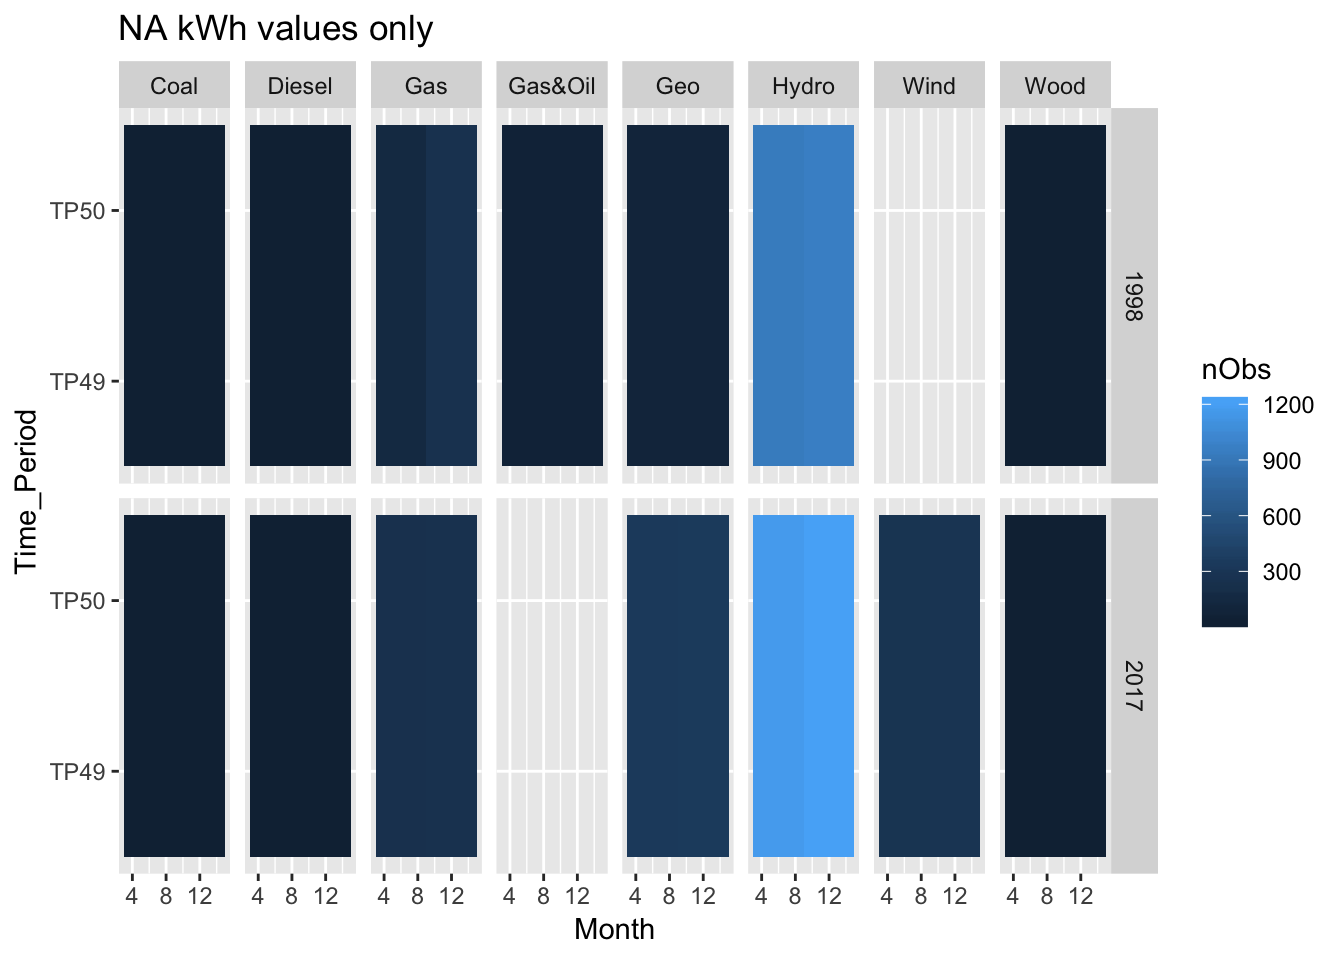
\includegraphics{nzElecGenTrends_files/figure-latex/exploreNA-1.pdf}
\caption{\label{fig:exploreNA}Plot showing presence of NA observations by
time period and Fuel Type}
\end{figure}

In order to avoid future confusion and to save a lot of error checking
we therefore remove NA kWh (i.e.~TP49 \& TP 50) from the dataset.

\begin{Shaded}
\begin{Highlighting}[]
\CommentTok{# N rows before:}
\KeywordTok{nrow}\NormalTok{(sampleGenDT)}
\end{Highlighting}
\end{Shaded}

\begin{verbatim}
## [1] 352250
\end{verbatim}

\begin{Shaded}
\begin{Highlighting}[]
\CommentTok{# N time periods before:}
\KeywordTok{uniqueN}\NormalTok{(sampleGenDT}\OperatorTok{$}\NormalTok{Time_Period)}
\end{Highlighting}
\end{Shaded}

\begin{verbatim}
## [1] 50
\end{verbatim}

\begin{Shaded}
\begin{Highlighting}[]
\CommentTok{# remove NA}
\NormalTok{sampleGenDT <-}\StringTok{ }\NormalTok{sampleGenDT[}\OperatorTok{!}\KeywordTok{is.na}\NormalTok{(kWh)]}
\CommentTok{# N rows after}
\KeywordTok{nrow}\NormalTok{(sampleGenDT)}
\end{Highlighting}
\end{Shaded}

\begin{verbatim}
## [1] 338160
\end{verbatim}

\begin{Shaded}
\begin{Highlighting}[]
\CommentTok{# N time periods after:}
\KeywordTok{uniqueN}\NormalTok{(sampleGenDT}\OperatorTok{$}\NormalTok{Time_Period)}
\end{Highlighting}
\end{Shaded}

\begin{verbatim}
## [1] 48
\end{verbatim}

\section{Analysis: 1998 \& 2017
Comparison}\label{analysis-1998-2017-comparison}

\subsection{Distribution tests}\label{distribution-tests}

Table \ref{tab:boxPlot} shows summary statistics for each fuel source by
year. Hydro contributes the majority of energy in each year but coal has
the highest half-hourly mean in each year suggesting that is makes large
contributions at specific times. Comparing the mean and median for coal
shows how skewed this distirbution was in 1998 although far less so in
2017. This is also supported by the maximum values which show coal as
the `peaked' energy producer in 1998 although this has faded by 2017
where it shows similar maxima to gas and hydro. Note that 2 of the 4 the
Huntly coal-fired units were
\href{https://en.wikipedia.org/wiki/Huntly_Power_Station}{mothballed/retired}
during this period.

Figure \ref{fig:boxPlot} shows the distribution of half-hourly
observations by month and year. It clearly shows the use of coal in June
1998, non-use in December 1998 but re-use in December 2017 where there
appears little differnece between winter \& summer use for most fuels.
We also see the emergence of wind by 2017.

\begin{table}

\caption{\label{tab:boxPlot}Summary of energy produced by all fuels}
\centering
\begin{tabular}[t]{r|l|r|r|r|r|r|r}
\hline
year & Fuel\_Code & sumMWh & meanMWh & medianMWh & minMWh & maxMWh & sdMWh\\
\hline
1998 & Coal & 379460.72 & 129.60 & 40.99 & 0 & 493.02 & 159.50\\
\hline
1998 & Diesel & 322.77 & 0.11 & 0.00 & 0 & 84.86 & 2.97\\
\hline
1998 & Gas & 537031.60 & 28.11 & 10.27 & 0 & 267.10 & 45.45\\
\hline
1998 & Gas\&Oil & 514797.99 & 87.91 & 91.95 & 0 & 173.73 & 43.46\\
\hline
1998 & Geo & 340786.48 & 38.80 & 25.60 & 0 & 81.87 & 28.90\\
\hline
1998 & Hydro & 3870532.38 & 42.64 & 26.49 & 0 & 294.98 & 53.53\\
\hline
1998 & Wood & 29067.50 & 9.93 & 14.10 & 0 & 19.50 & 7.41\\
\hline
2017 & Coal & 426606.86 & 145.70 & 140.41 & 0 & 241.88 & 64.98\\
\hline
2017 & Diesel & 941.40 & 0.32 & 0.00 & 0 & 45.39 & 2.49\\
\hline
2017 & Gas & 1367101.27 & 58.36 & 22.78 & 0 & 290.87 & 75.67\\
\hline
2017 & Geo & 1222782.96 & 37.97 & 38.87 & 0 & 84.75 & 23.46\\
\hline
2017 & Hydro & 3586485.42 & 31.41 & 19.57 & 0 & 291.82 & 39.68\\
\hline
2017 & Wind & 255368.77 & 9.73 & 6.30 & 0 & 44.27 & 9.90\\
\hline
2017 & Wood & 43571.23 & 14.88 & 16.64 & 0 & 19.51 & 4.91\\
\hline
\end{tabular}
\end{table}

\begin{figure}
\centering
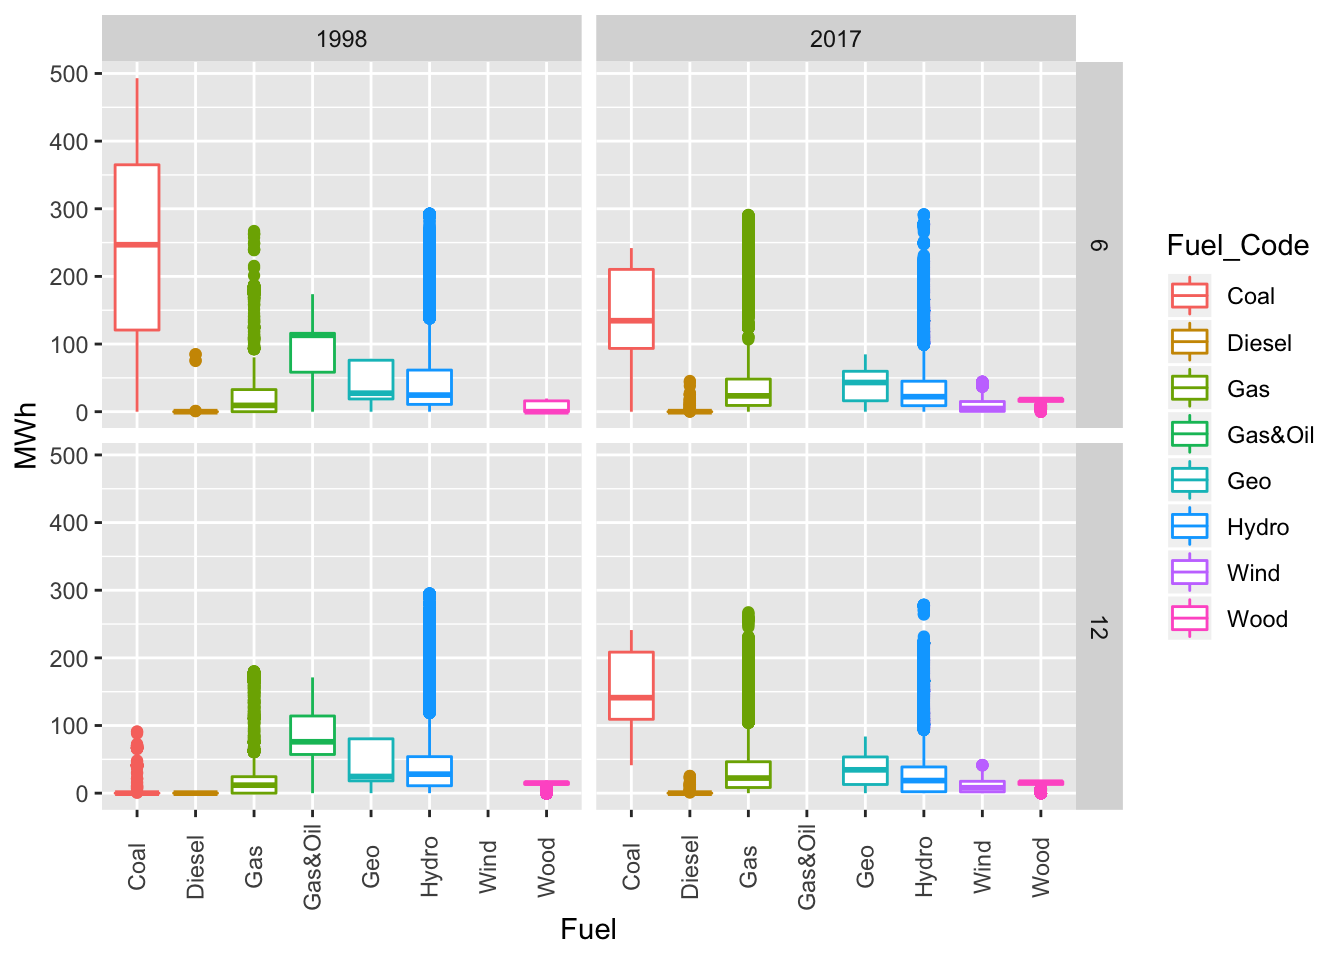
\includegraphics{nzElecGenTrends_files/figure-latex/boxPlot-1.pdf}
\caption{\label{fig:boxPlot}Box plot of energy produced by all fuels}
\end{figure}

Figure \ref{fig:overallHistograms} visualises the distribution of MWh
values within fuel sources. Note that the vertical axis has been allowed
to vary by fuel source so that smaller counts are visible. The y axis is
constant which enables the higher unit output of coal to be clearly
visible. The histogram for coal shows the use of multiple units in June
1998 but not 2017 for example where the output is clearly truncated. It
also shows that coal was almost constantly generating in 2017 (very few
zero values). Hydro on the other hand shows a large number of zero or
low values as does wind and back-up diesel which is to be expected.

\begin{figure}
\centering
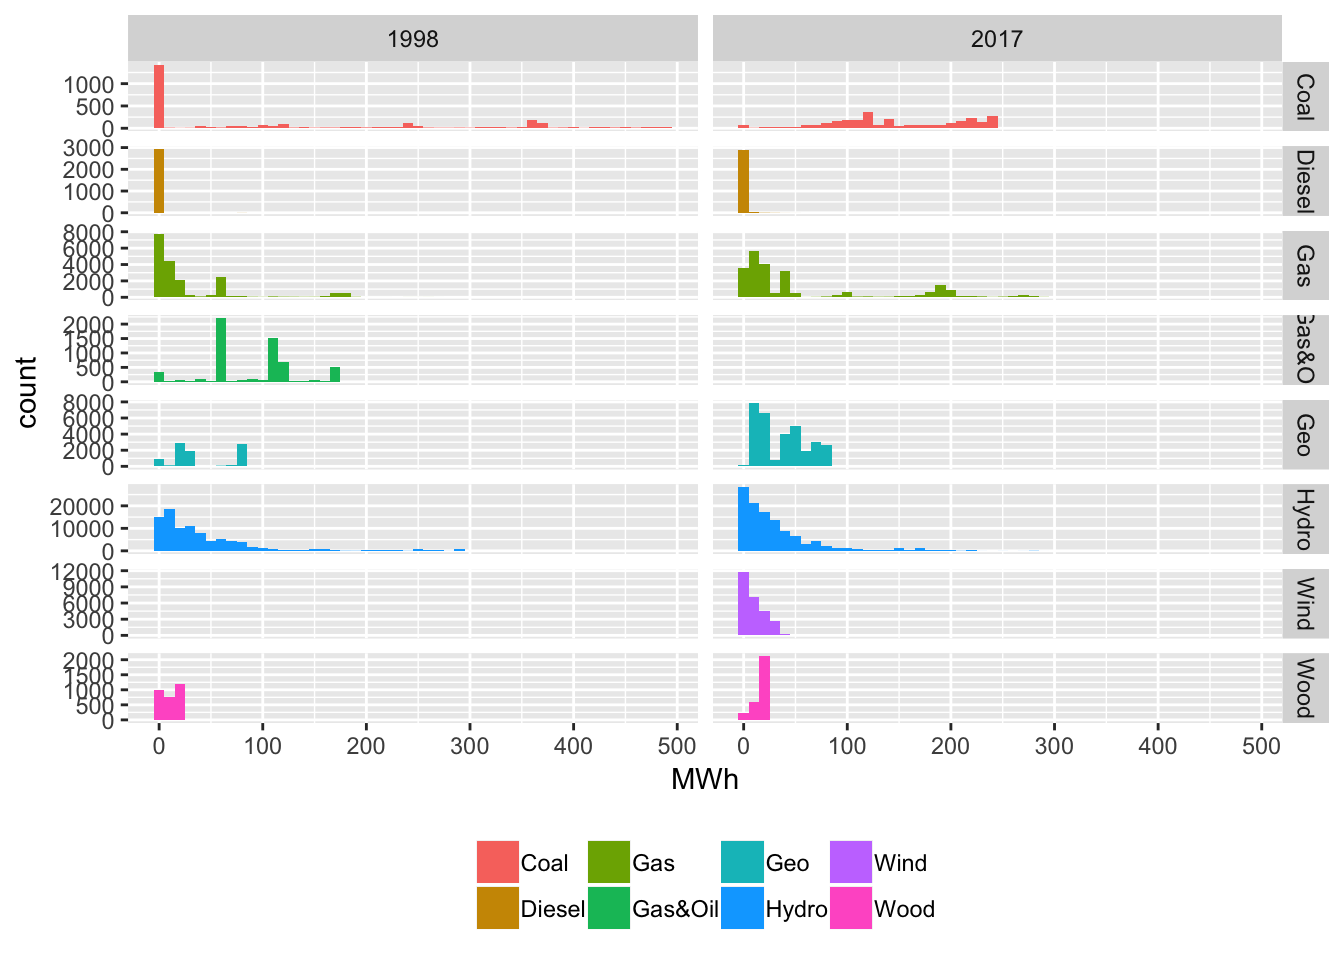
\includegraphics{nzElecGenTrends_files/figure-latex/overallHistograms-1.pdf}
\caption{\label{fig:overallHistograms}Overall energy production histrograms
by fuel type}
\end{figure}

\subsection{Monthly generation}\label{monthly-generation}

The following plots shows the total, mean, s.d. and coefficient of
variation plots of half-hourly GWh produced by each fuel source each
month and to some extent relfects the previous box plots.

The total is simply the sum of all half-hourly values and Figure
\ref{fig:monthlyTotalPlot} shows the dominance of hydro followed by coal
in June 1998; the non-use of coal in December 1998; the growth of gas \&
geo by 2017 but the relative stasis in at-capacity hydro (?).

\begin{figure}
\centering
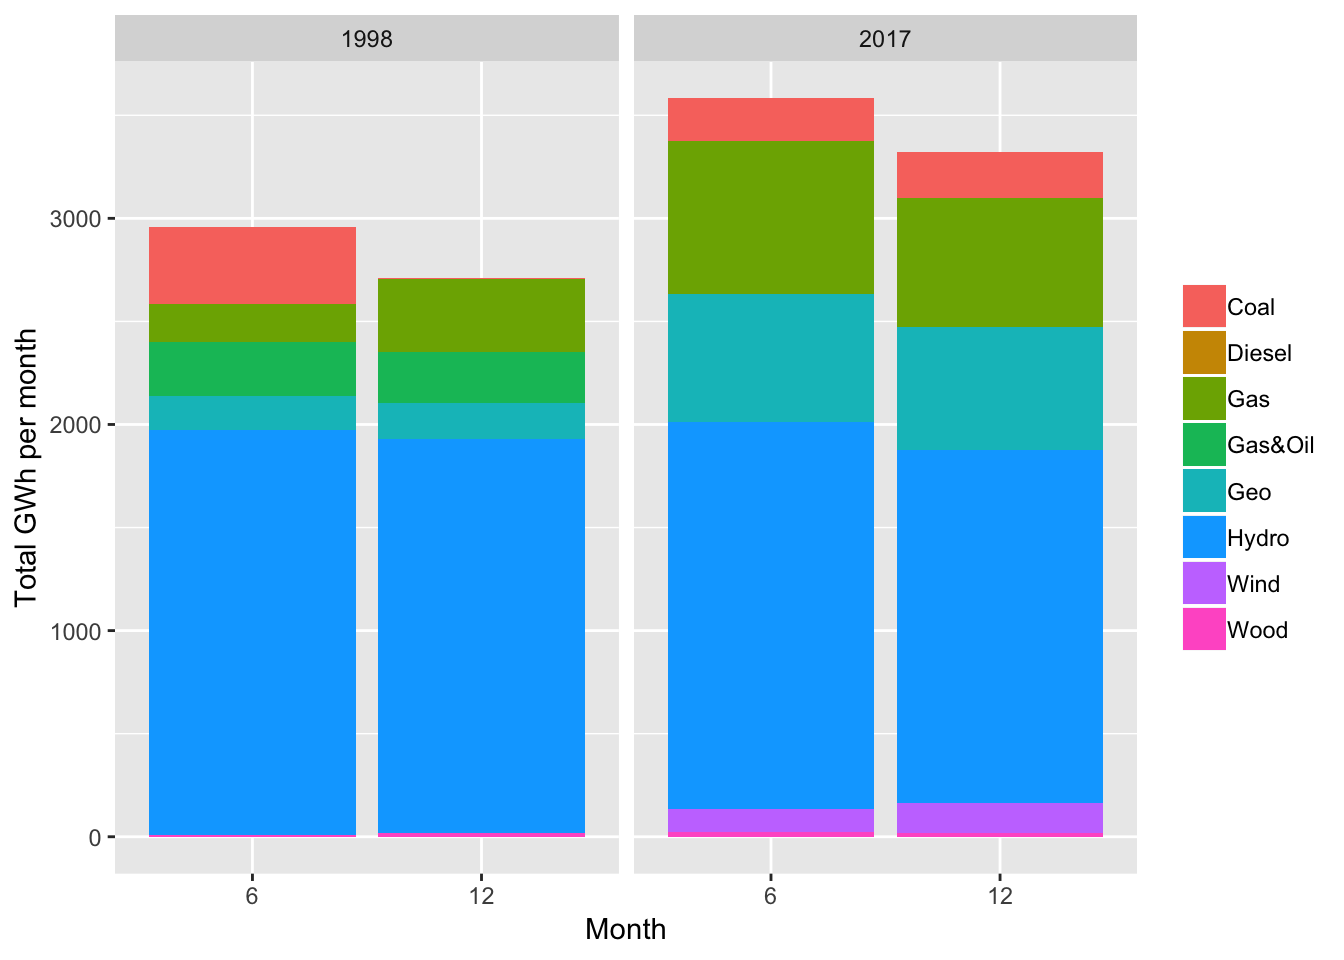
\includegraphics{nzElecGenTrends_files/figure-latex/monthlyTotalPlot-1.pdf}
\caption{\label{fig:monthlyTotalPlot}Monthly total plot by fuel type}
\end{figure}

Figure \ref{fig:monthlyMeanPlot} shows the mean of half-hourly values
for each month and indicates that the Coal generation may be skewed,
especially for June 1998 by a few very large values (ref the histograms
above).
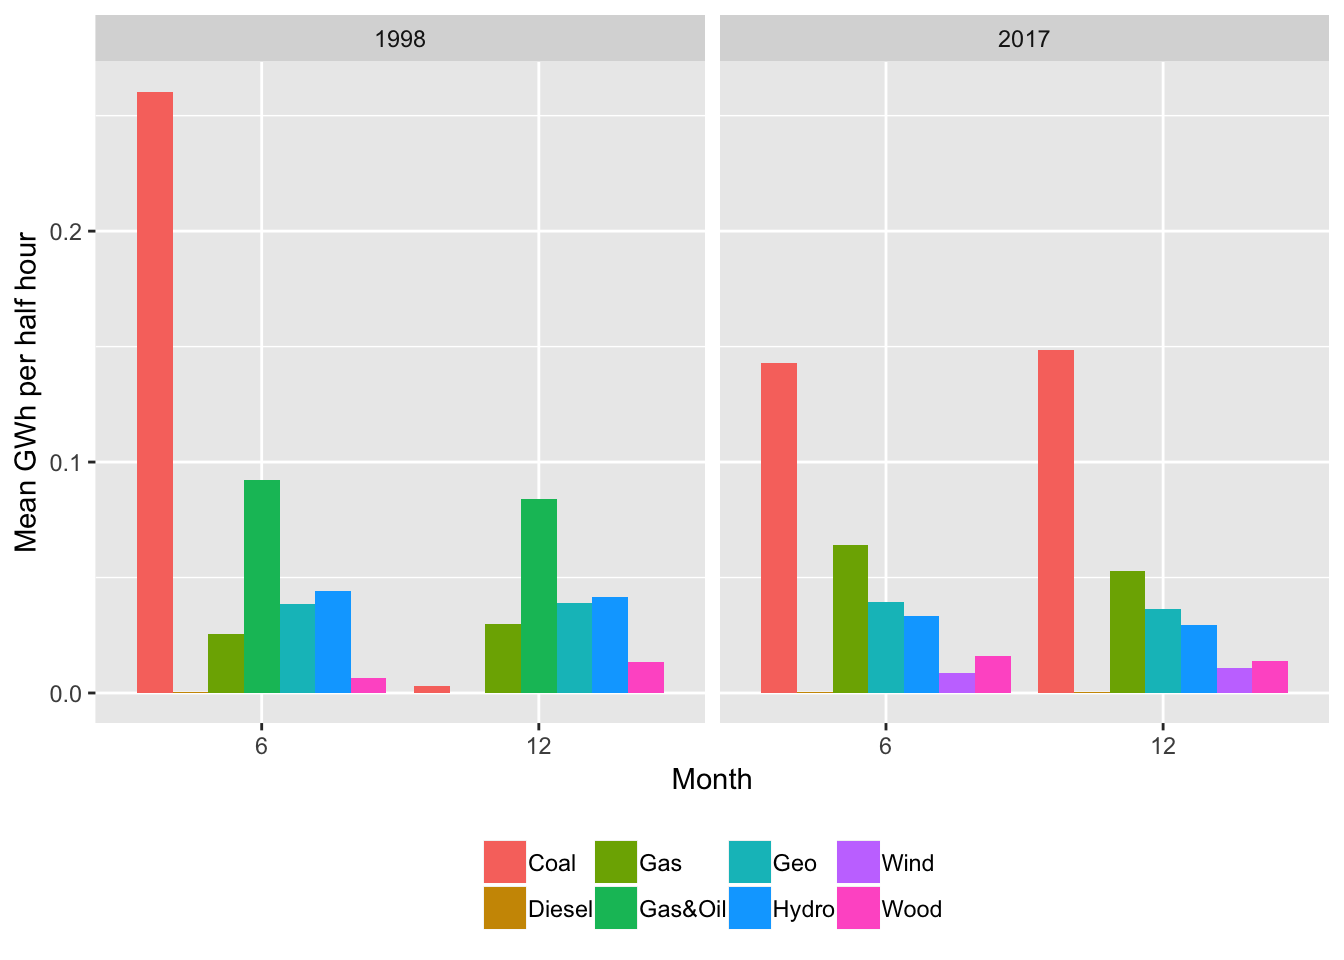
\includegraphics{nzElecGenTrends_files/figure-latex/monthlyMeanPlot-1.pdf}

Figure \ref{fig:monthlySdPlot} shows the standard deviation of the
half-hourly generation data and suggests that coal has the highest
absolute variation in June 1998 which may correspond to a particular
spike and/or a period of very heavy use. Coal is less variable in 2017
perhaps due to the increased use of Gas.

\begin{figure}
\centering
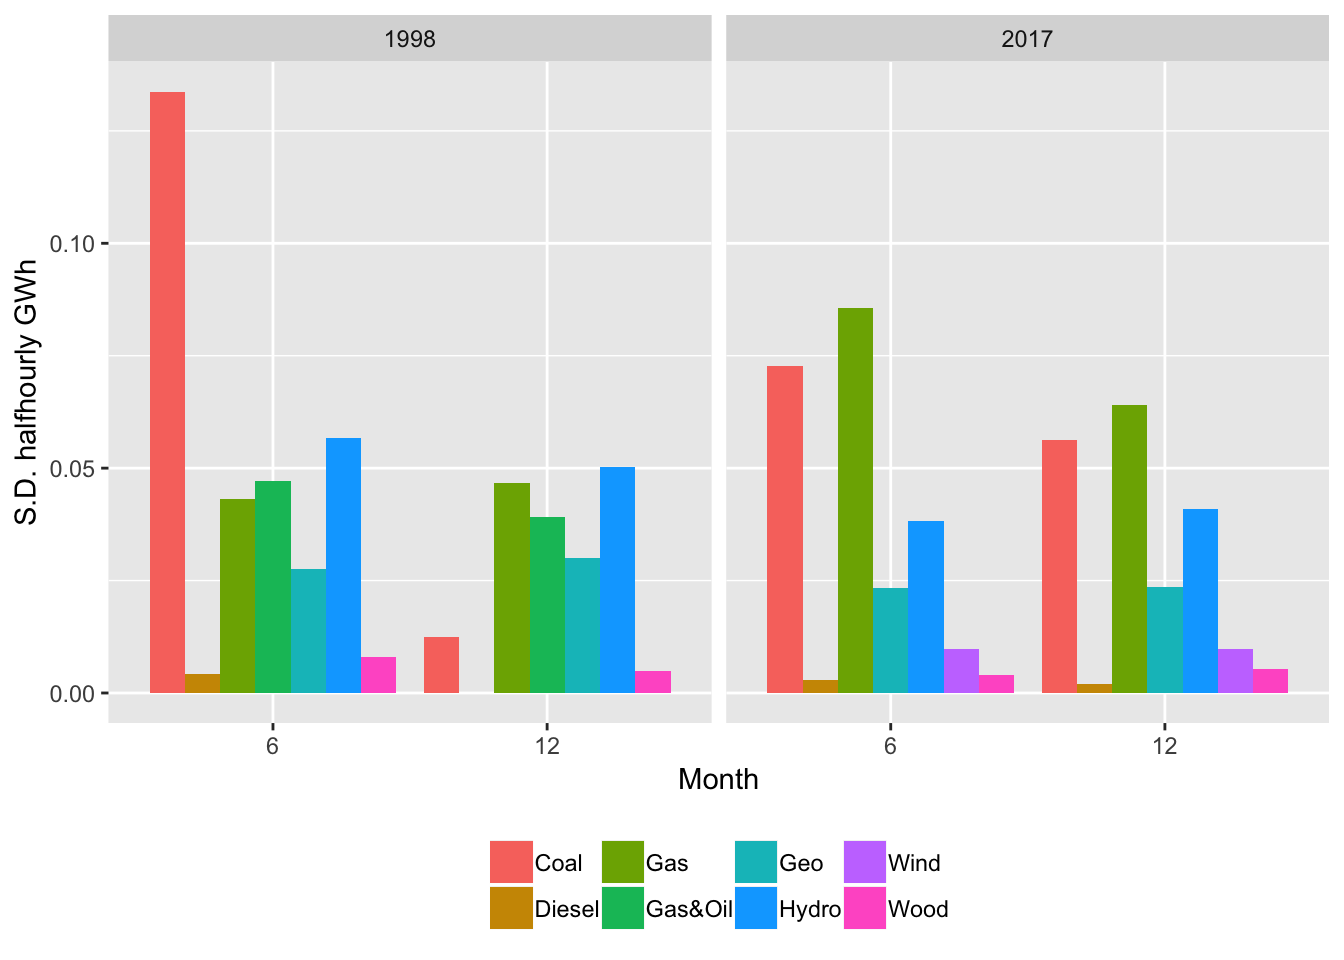
\includegraphics{nzElecGenTrends_files/figure-latex/monthlySdPlot-1.pdf}
\caption{\label{fig:monthlySdPlot}Monthly s.d. plot by fuel type}
\end{figure}

Finally, Figure \ref{fig:monthlyCovPlot} shows the coefficient of
variation across the half-hourly values (mean/s.d). We take the CoV to
indicate \emph{relative} variability (i.e.~relative volatility) in
generation load between the different fuels and use it in preference to
the standard deviation (shown above) which, as an absolute measure, is
affected by the underlying magnitude of each fuel's use. The plots
suggest that Coal and Wood tend to see greatest relative variability
although Gas \& Oil in 1998 also stand out.

\begin{Shaded}
\begin{Highlighting}[]
\CommentTok{# coefficient of variation https://en.wikipedia.org/wiki/Coefficient_of_variation}
\NormalTok{plotDT <-}\StringTok{ }\NormalTok{plotDT[, cov }\OperatorTok{:}\ErrorTok{=}\StringTok{ }\DecValTok{1000000} \OperatorTok{*}\StringTok{ }\NormalTok{(meankWh}\OperatorTok{/}\NormalTok{sdkWh)] }\CommentTok{# corrct for GW conversion in plot function (doh!)}

\KeywordTok{makeMonthlyDodgedPlot}\NormalTok{(plotDT, }\StringTok{"cov"}\NormalTok{, }\StringTok{"CoV half-hourly GWh"}\NormalTok{) }\OperatorTok{+}\StringTok{ }\KeywordTok{geom_col}\NormalTok{(}\DataTypeTok{position =} \StringTok{"dodge"}\NormalTok{)}
\end{Highlighting}
\end{Shaded}

\begin{verbatim}
## Warning: Removed 1 rows containing missing values (geom_col).

## Warning: Removed 1 rows containing missing values (geom_col).
\end{verbatim}

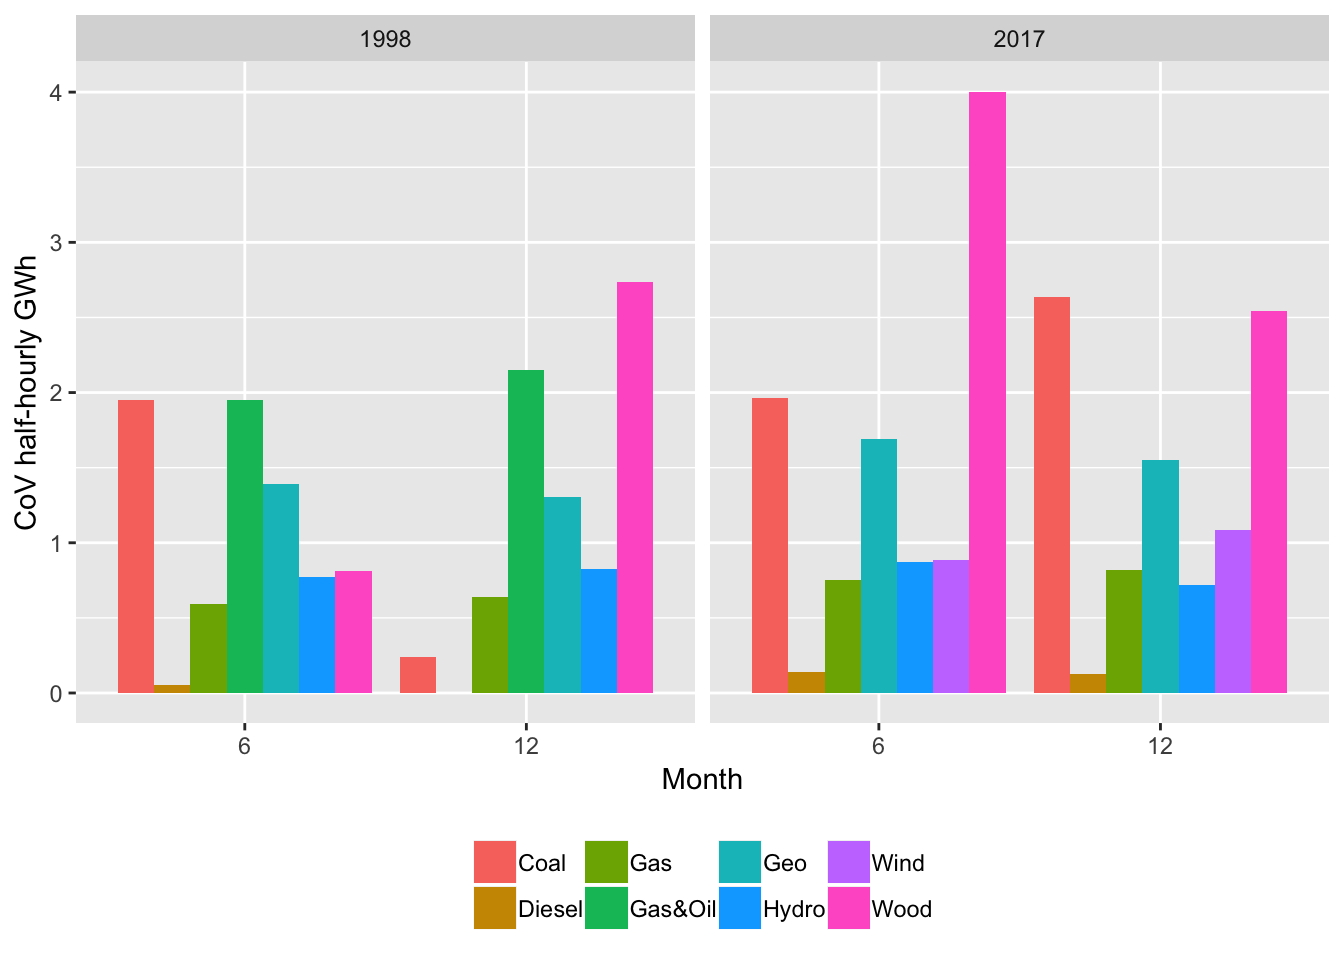
\includegraphics{nzElecGenTrends_files/figure-latex/monthlyCovPlot-1.pdf}

\subsection{Half hourly profiles by
month}\label{half-hourly-profiles-by-month}

However the monthly plots do not tell us about the use of different
generation sources by time of day which has clear implications for how
peaks in demand have been met over time.

To do this, the following plots partially replicate one of those found
in
\href{https://www.sciencedirect.com/science/article/pii/S0301421516307017\#f0025}{Staffel,
2018} for the UK to show how the different components of generation have
changed over time.

Figure \ref{fig:sumProfileCol} shows the total half-hourly generation
for each month summed over all days whilst Figure
\ref{fig:sumProfilePoint} shows the same data but as a point plot to
more clearly show the absolute contribution of each fuel. Note that the
half-hours are plotted at mid-points (00:15, 00:45, 01:15 etc\ldots{}).

\begin{figure}
\centering
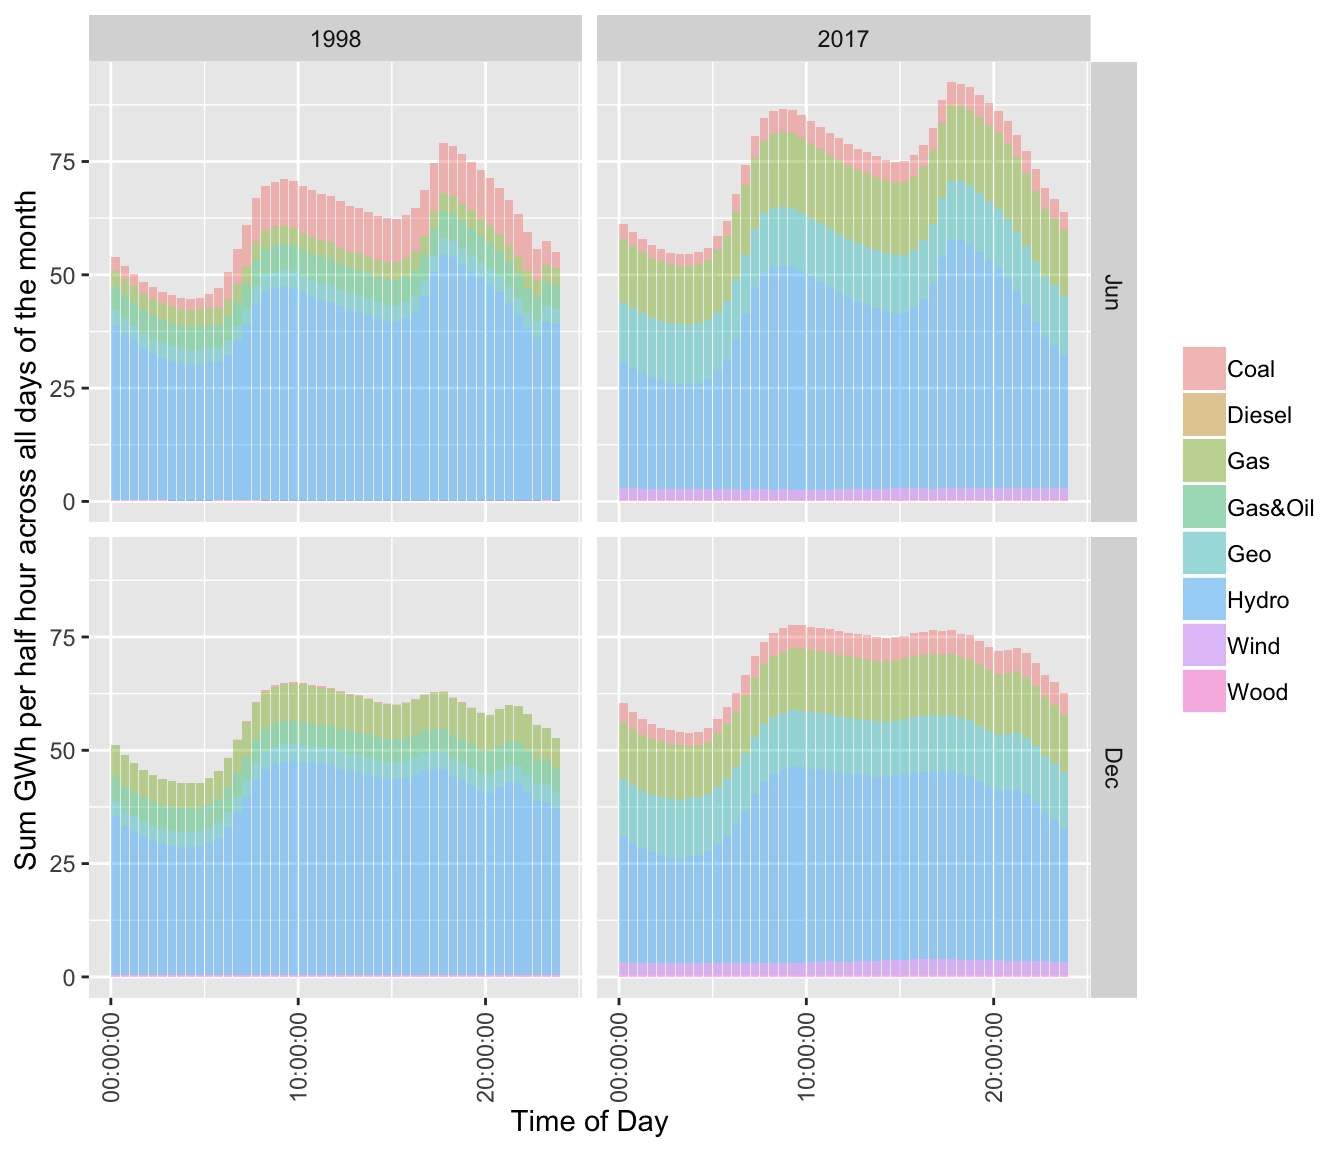
\includegraphics{nzElecGenTrends_files/figure-latex/sumProfileCol-1.pdf}
\caption{\label{fig:sumProfileCol}Half-hourly profile plot by fuel type
(sum)}
\end{figure}

\begin{figure}
\centering
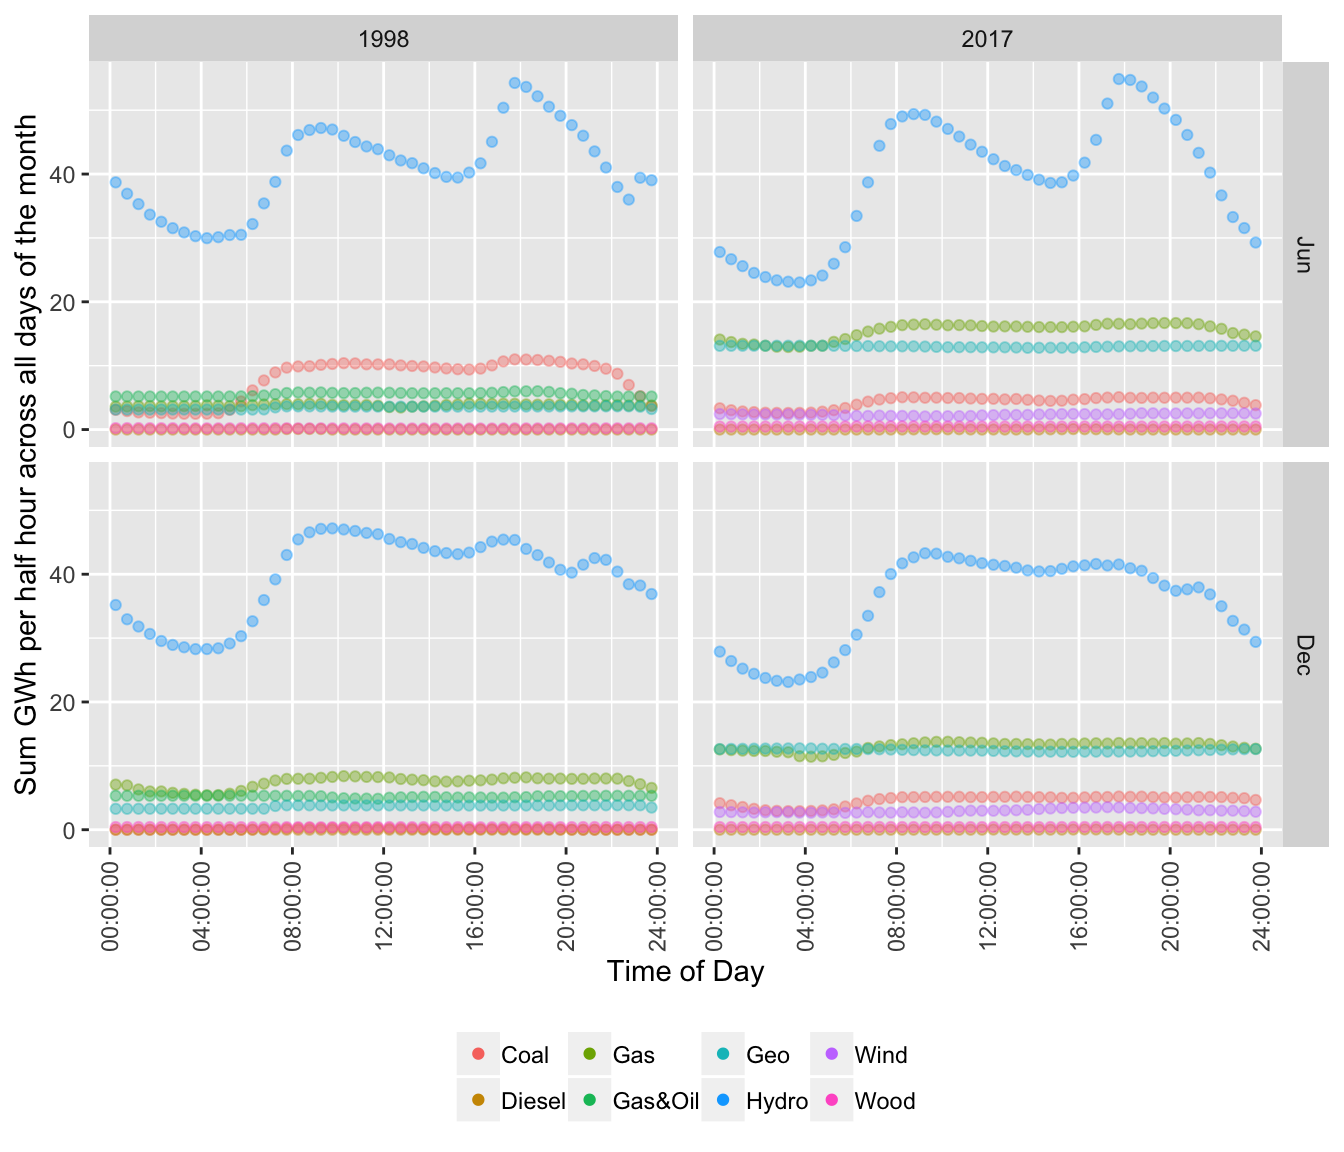
\includegraphics{nzElecGenTrends_files/figure-latex/sumProfilePoint-1.pdf}
\caption{\label{fig:sumProfilePoint}Half-hourly profile plot by fuel type
(sum)}
\end{figure}

Figures \ref{fig:meanProfileCol} and \ref{fig:meanProfilePoint} repeat
this analysis but shows the mean, again suggesting that the values for
coal are skewed by some extremely large values in December 1998 and by
high generation values when used in 2017.

\begin{figure}
\centering
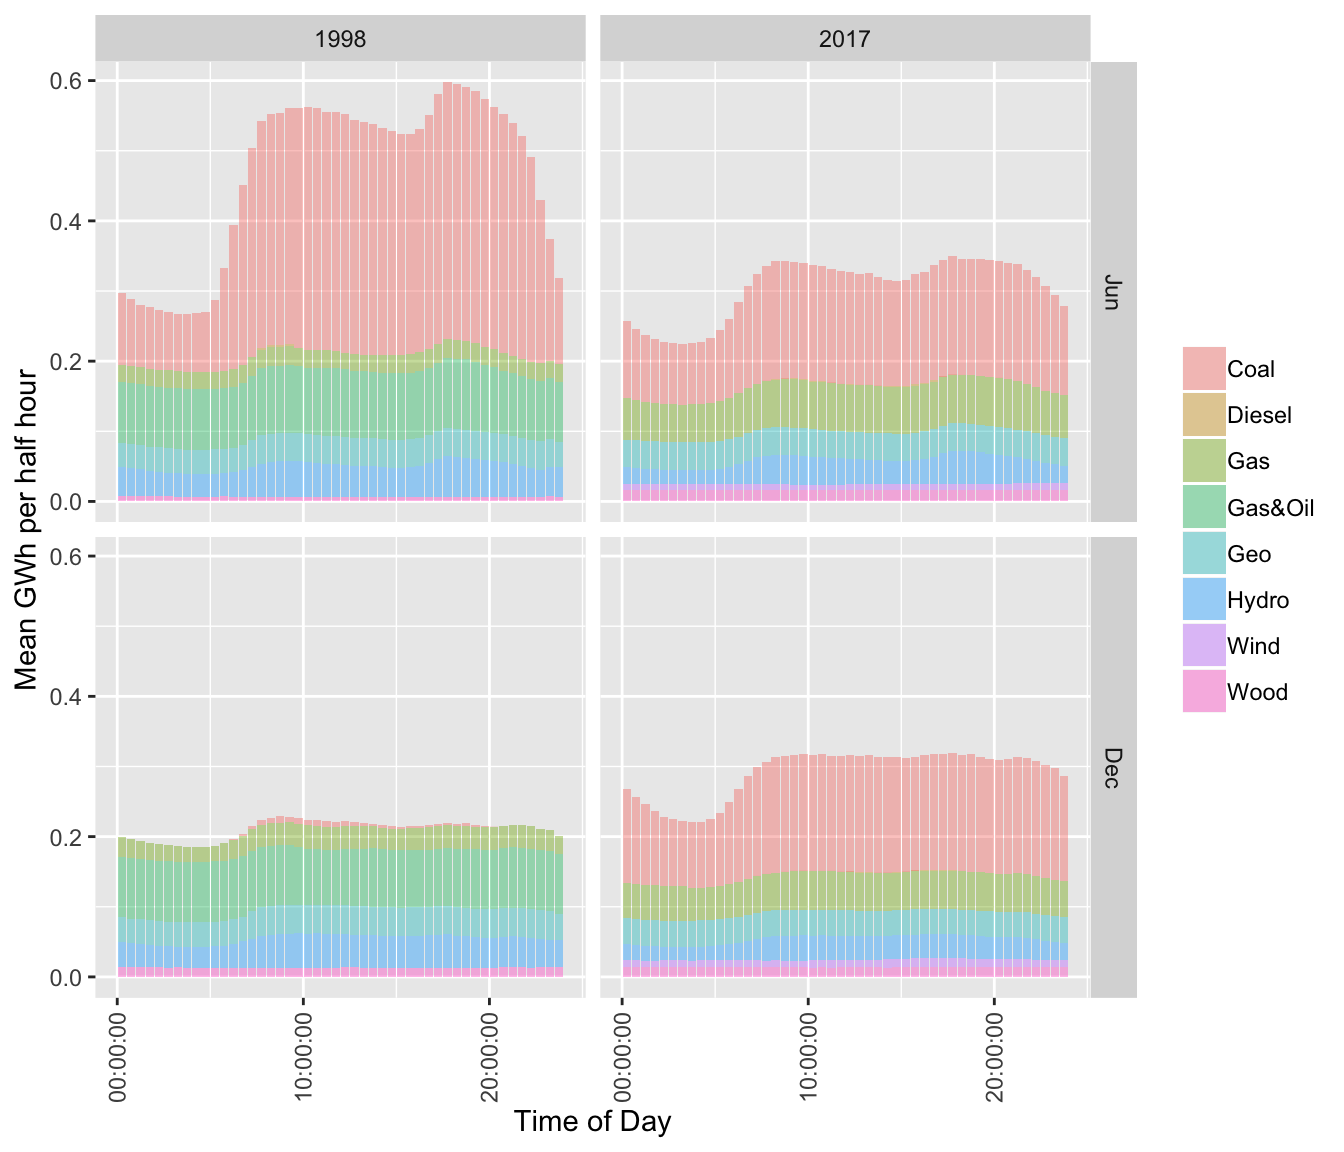
\includegraphics{nzElecGenTrends_files/figure-latex/meanProfileCol-1.pdf}
\caption{\label{fig:meanProfileCol}Half-hourly profile plot by fuel type
(mean)}
\end{figure}

\begin{figure}
\centering
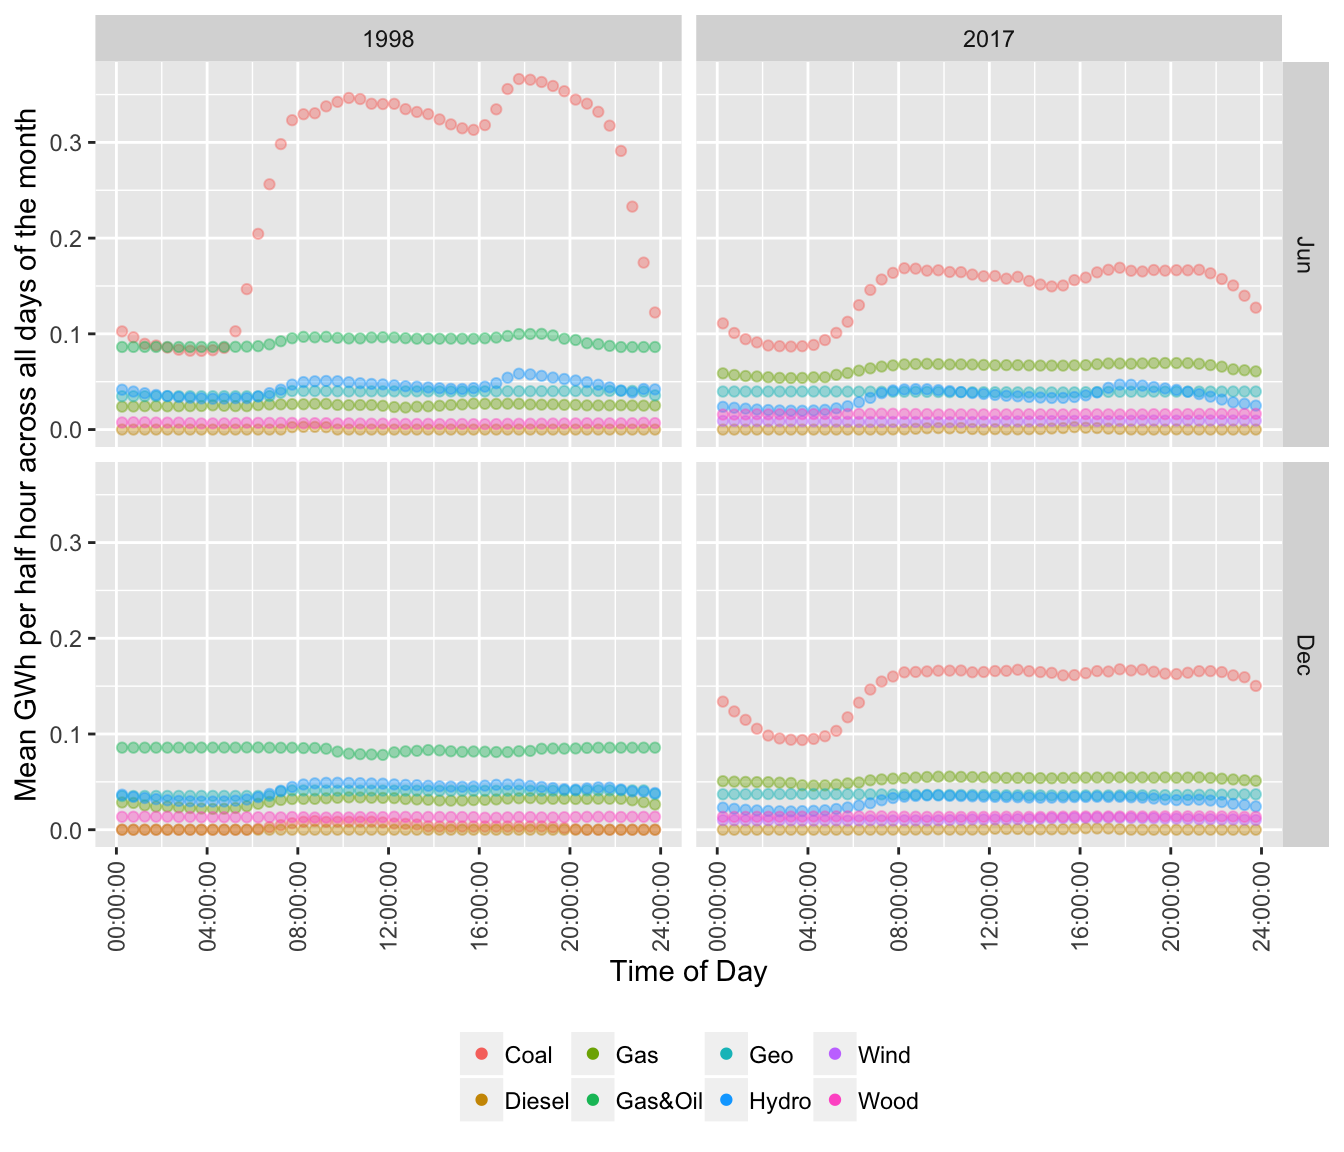
\includegraphics{nzElecGenTrends_files/figure-latex/meanProfilePoint-1.pdf}
\caption{\label{fig:meanProfilePoint}Half-hourly profile plot by fuel type
(mean)}
\end{figure}

\subsection{Half hourly profiles by day of the
month}\label{half-hourly-profiles-by-day-of-the-month}

The following plots show the profiles for each day of the month.
Unfortunately due to the lack of wind generation in 1998 the colour
scheme changes from 1998 to 2017.

\begin{quote}
To be fixed
\end{quote}

Nevertheless the differences between the compositions of each half-hour
can be seen.

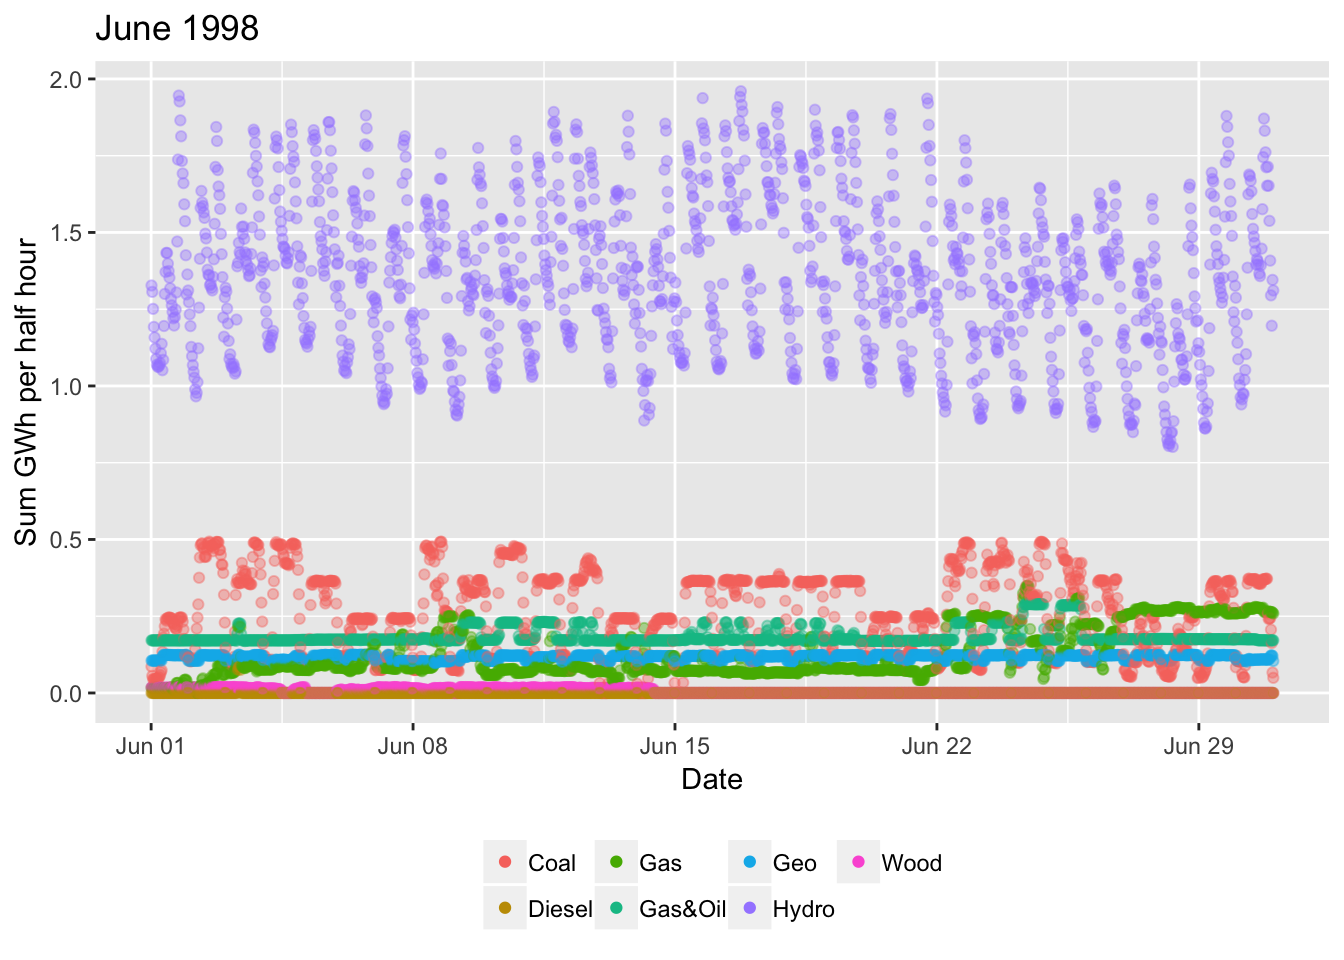
\includegraphics{nzElecGenTrends_files/figure-latex/sumDailyProfilePoint-1.pdf}
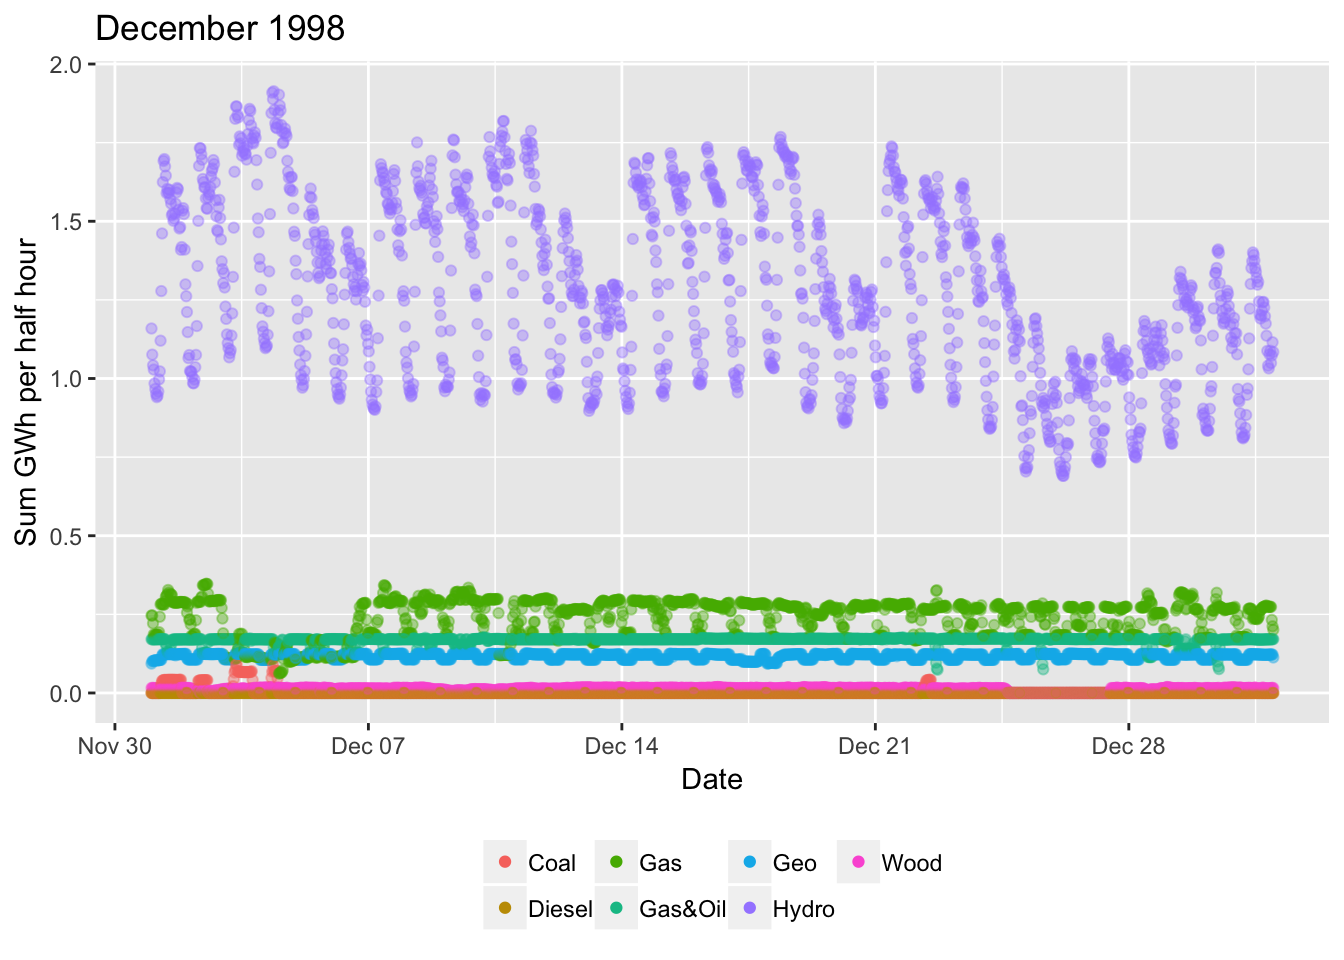
\includegraphics{nzElecGenTrends_files/figure-latex/sumDailyProfilePoint-2.pdf}
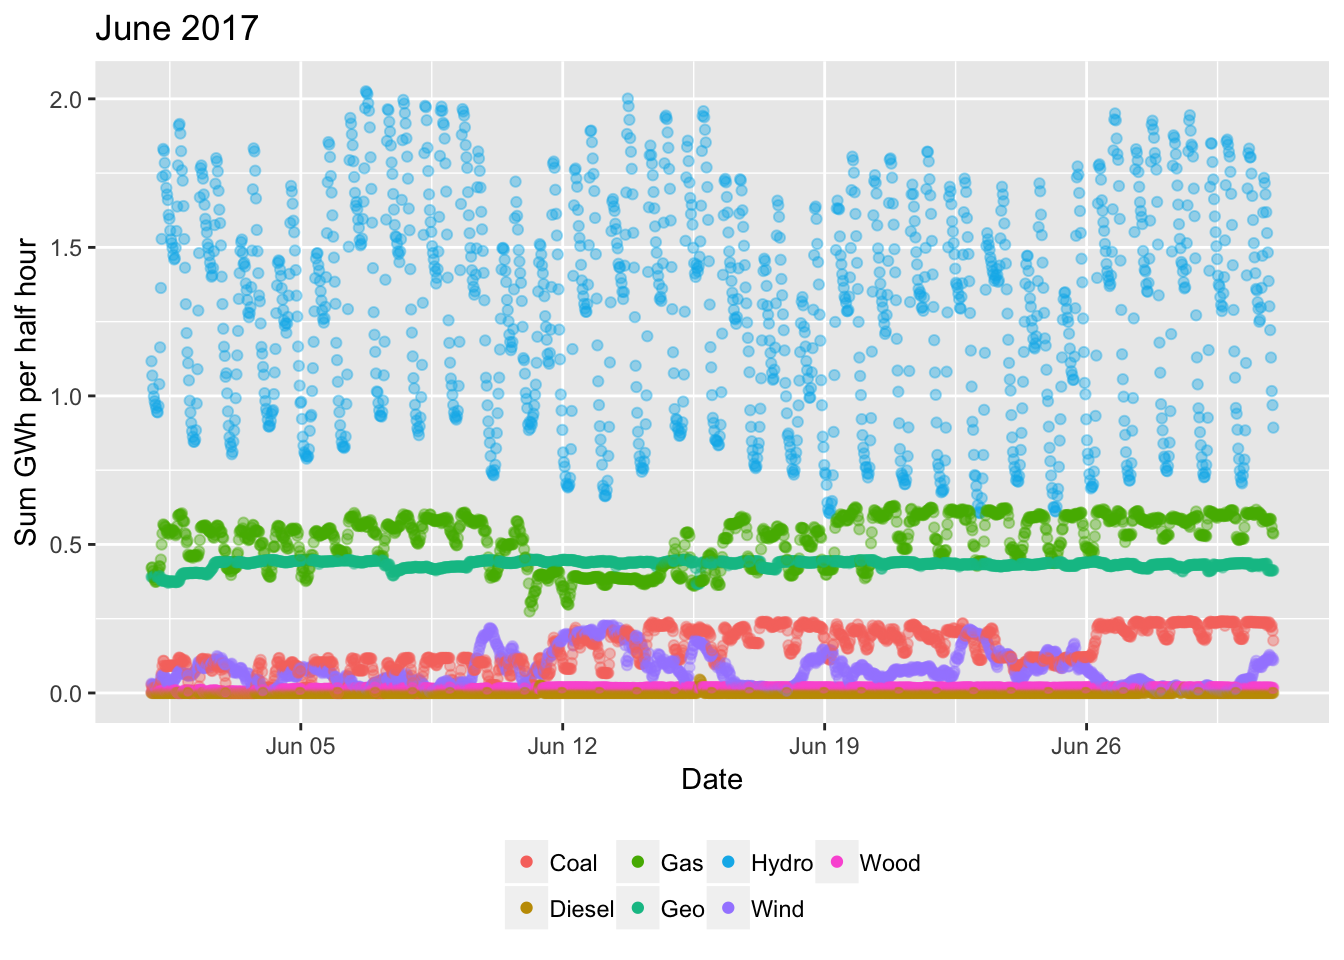
\includegraphics{nzElecGenTrends_files/figure-latex/sumDailyProfilePoint-3.pdf}
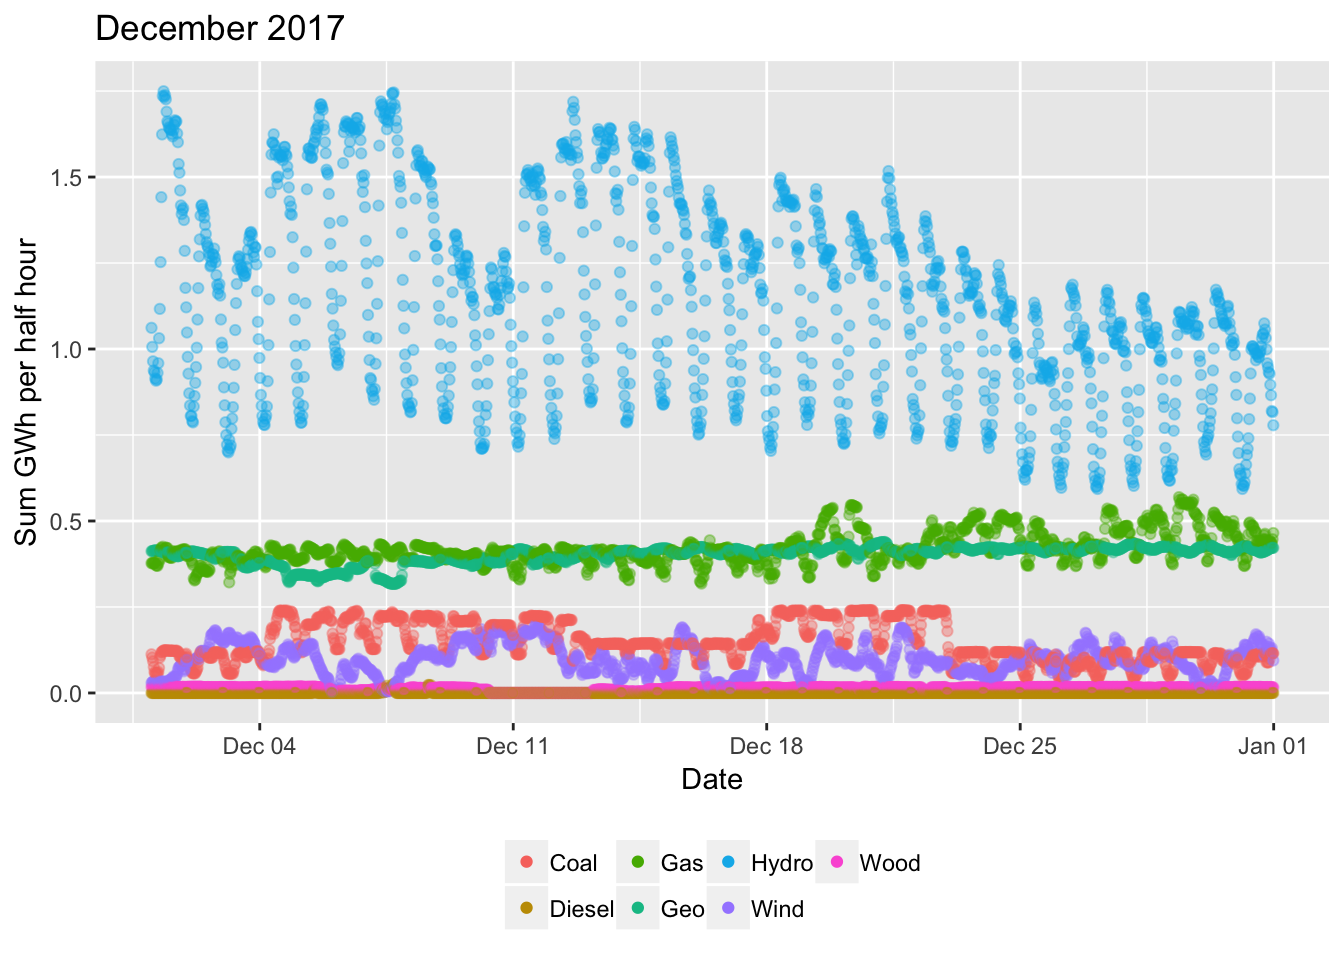
\includegraphics{nzElecGenTrends_files/figure-latex/sumDailyProfilePoint-4.pdf}

Figure \ref{fig:sumDailyProfilePoint} shows the total as a point plot
while Figure \ref{fig:sumDailyProfileCol} shows the total as stacked
column plots to show the proportion of energy generation produced by
each fuel.

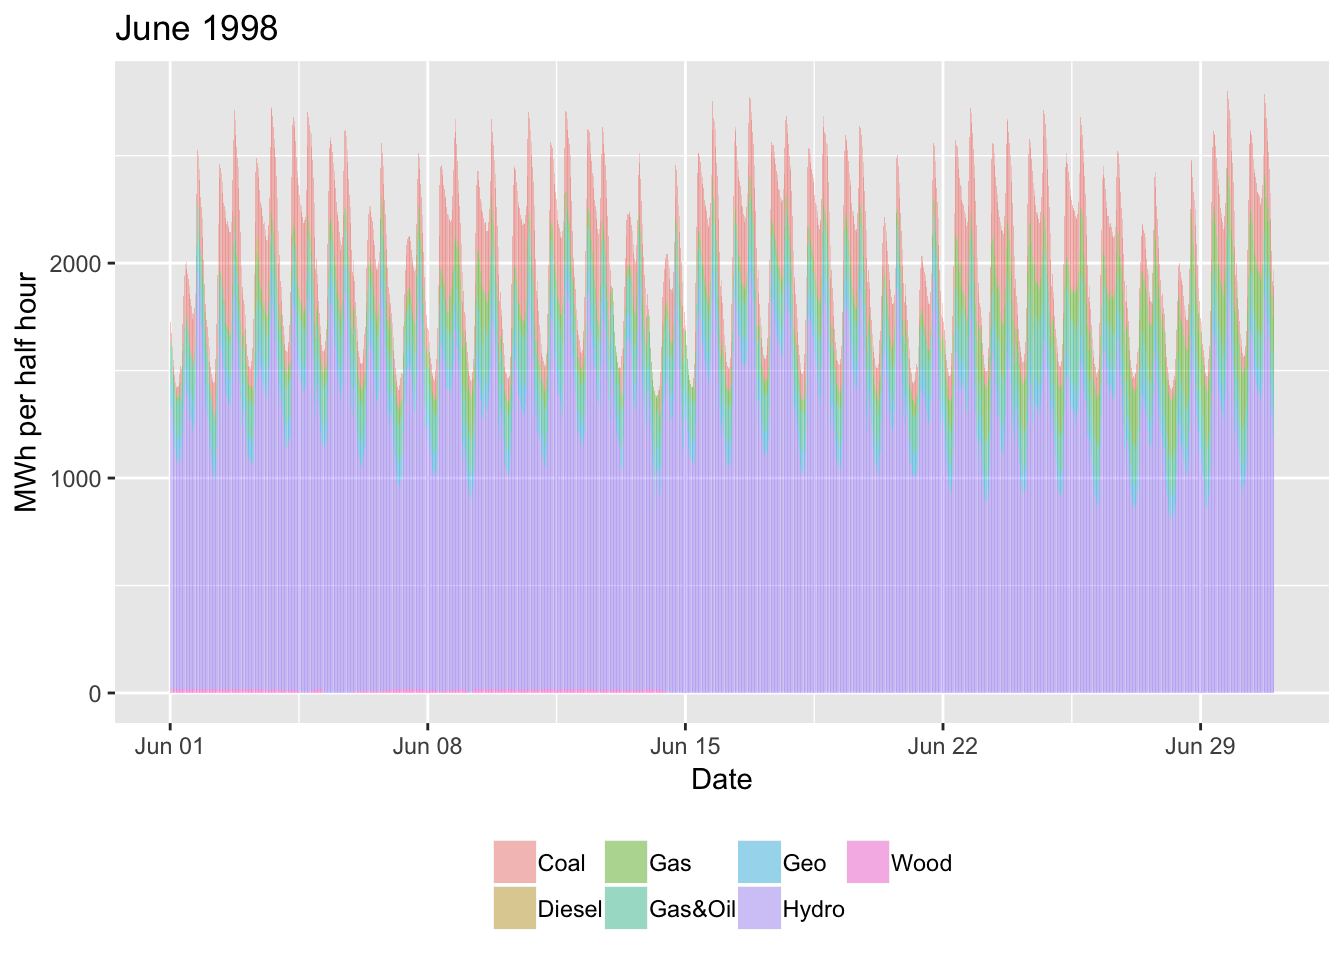
\includegraphics{nzElecGenTrends_files/figure-latex/sumDailyProfileCol-1.pdf}
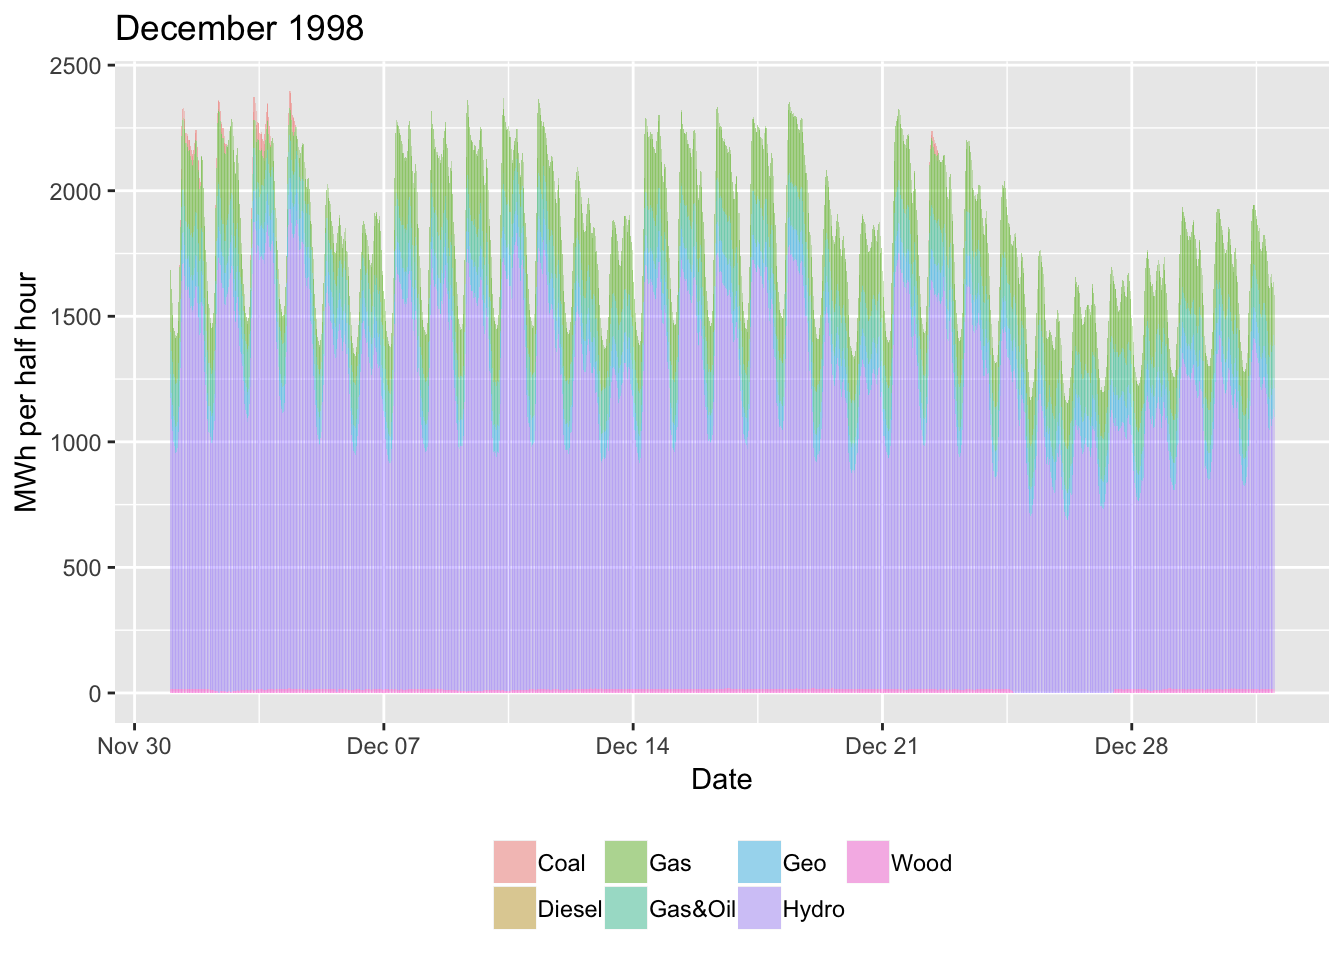
\includegraphics{nzElecGenTrends_files/figure-latex/sumDailyProfileCol-2.pdf}
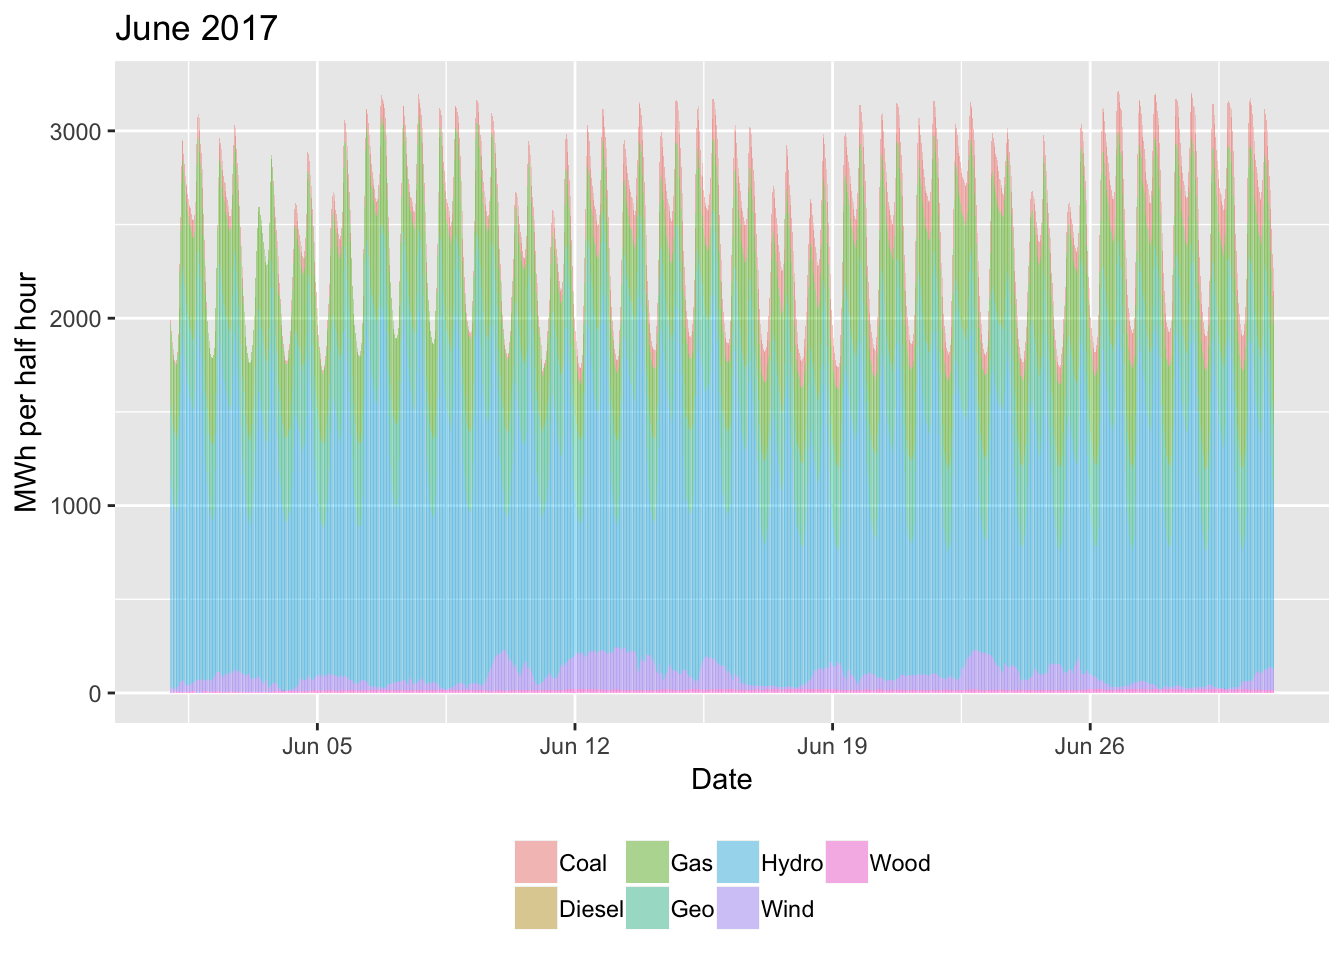
\includegraphics{nzElecGenTrends_files/figure-latex/sumDailyProfileCol-3.pdf}
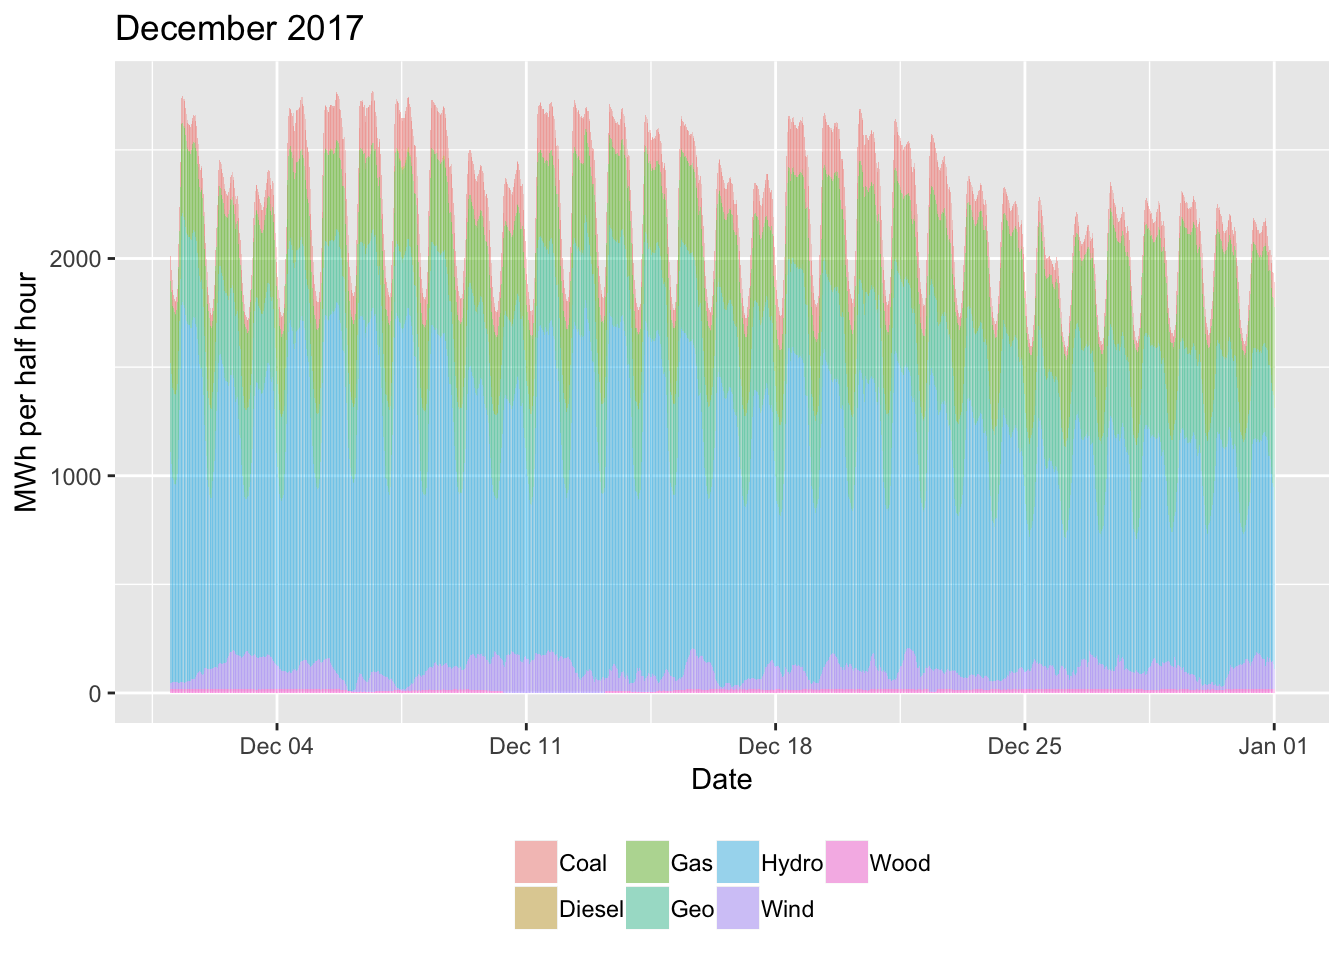
\includegraphics{nzElecGenTrends_files/figure-latex/sumDailyProfileCol-4.pdf}

\section{Analysis: Trends 1998 -
2017}\label{analysis-trends-1998---2017}

Using full dataset for each day, month \& year.

\begin{verbatim}
## [1] "Files loaded"
\end{verbatim}

\begin{verbatim}
## [1] "Loaded 22,503,700 rows of data"
\end{verbatim}

As above, in order to avoid future confusion and to save a lot of error
checking we again remove NA kWh (i.e.~TP49 \& TP 50) from the dataset.

\begin{Shaded}
\begin{Highlighting}[]
\CommentTok{# N rows before:}
\KeywordTok{nrow}\NormalTok{(allGenDT)}
\end{Highlighting}
\end{Shaded}

\begin{verbatim}
## [1] 22503700
\end{verbatim}

\begin{Shaded}
\begin{Highlighting}[]
\CommentTok{# N time periods before:}
\KeywordTok{uniqueN}\NormalTok{(allGenDT}\OperatorTok{$}\NormalTok{Time_Period)}
\end{Highlighting}
\end{Shaded}

\begin{verbatim}
## [1] 50
\end{verbatim}

\begin{Shaded}
\begin{Highlighting}[]
\CommentTok{# remove NA}
\NormalTok{allGenDT <-}\StringTok{ }\NormalTok{allGenDT[}\OperatorTok{!}\KeywordTok{is.na}\NormalTok{(kWh)]}
\CommentTok{# N rows after}
\KeywordTok{nrow}\NormalTok{(allGenDT)}
\end{Highlighting}
\end{Shaded}

\begin{verbatim}
## [1] 21600076
\end{verbatim}

\begin{Shaded}
\begin{Highlighting}[]
\CommentTok{# N time periods after:}
\KeywordTok{uniqueN}\NormalTok{(allGenDT}\OperatorTok{$}\NormalTok{Time_Period)}
\end{Highlighting}
\end{Shaded}

\begin{verbatim}
## [1] 50
\end{verbatim}

\subsection{Trends over years}\label{trends-over-years}

The hydro trends (and the consequences for Carbon-based generation)
should be seen in the context of the
\href{https://www.niwa.co.nz/climate/information-and-resources/elnino/el-nino-and-southern-oscillation}{Southern
Oscilation}'s effect on rainfall.

\begin{figure}
\centering
\includegraphics{https://www.niwa.co.nz/sites/niwa.co.nz/files/styles/sidebar/public/sites/default/files/images/imported/0005/73454/soi_5mthmn_188003-201509_v2.png}
\caption{Southern Oscillation Index}
\end{figure}

``Although El Niño and La Niña (collectively known as El Niño-Southern
Oscillation or ENSO) have an important influence on New Zealand's
climate, it accounts for less than 25 percent of the year-to year
variance in seasonal rainfall and temperature at most locations.
Nevertheless, its effects can be significant.''
\url{https://www.niwa.co.nz/climate/information-and-resources/elnino/elnino-impacts-on-newzealand}

``La Niña events have different impacts on New Zealand's climate. More
north--easterly winds are characteristic, which tend to bring moist,
rainy conditions to the north--east of the North Island, and reduced
rainfall to the south and south--west of the South Island.

Therefore, some areas, such as central Otago and South Canterbury, can
experience drought in both El Niño and La Niña. "

Figure \ref(fig:monthlySOI) shows the monthly El Niño Southern
Oscillation Index for 1986--2016 and shows at least four strong El Nino
periods centred on 1987, 1993, 1997, 2005 and 2015.

\begin{verbatim}
## Parsed with column specification:
## cols(
##   Month_year = col_character(),
##   Southern_oscillation_index = col_double()
## )
\end{verbatim}

\begin{verbatim}
##    Month_year Southern_oscillation_index
## 1:     Jan-86                        1.0
## 2:     Feb-86                       -1.0
## 3:     Mar-86                        0.5
## 4:     Apr-86                        0.3
## 5:     May-86                       -0.2
## 6:     Jun-86                        1.0
\end{verbatim}

\begin{verbatim}
## Warning in grid.Call(C_stringMetric, as.graphicsAnnot(x$label)): font
## metrics unknown for Unicode character U+2013

## Warning in grid.Call(C_stringMetric, as.graphicsAnnot(x$label)): font
## metrics unknown for Unicode character U+2013
\end{verbatim}

\begin{verbatim}
## Warning in grid.Call(C_stringMetric, as.graphicsAnnot(x$label)): conversion
## failure on 'Monthly El Niño Southern Oscillation Index, 1986–2016' in
## 'mbcsToSbcs': dot substituted for <e2>
\end{verbatim}

\begin{verbatim}
## Warning in grid.Call(C_stringMetric, as.graphicsAnnot(x$label)): conversion
## failure on 'Monthly El Niño Southern Oscillation Index, 1986–2016' in
## 'mbcsToSbcs': dot substituted for <80>
\end{verbatim}

\begin{verbatim}
## Warning in grid.Call(C_stringMetric, as.graphicsAnnot(x$label)): conversion
## failure on 'Monthly El Niño Southern Oscillation Index, 1986–2016' in
## 'mbcsToSbcs': dot substituted for <93>
\end{verbatim}

\begin{verbatim}
## Warning in grid.Call(C_textBounds, as.graphicsAnnot(x$label), x$x, x$y, :
## conversion failure on 'Monthly El Niño Southern Oscillation Index, 1986–
## 2016' in 'mbcsToSbcs': dot substituted for <e2>
\end{verbatim}

\begin{verbatim}
## Warning in grid.Call(C_textBounds, as.graphicsAnnot(x$label), x$x, x$y, :
## conversion failure on 'Monthly El Niño Southern Oscillation Index, 1986–
## 2016' in 'mbcsToSbcs': dot substituted for <80>
\end{verbatim}

\begin{verbatim}
## Warning in grid.Call(C_textBounds, as.graphicsAnnot(x$label), x$x, x$y, :
## conversion failure on 'Monthly El Niño Southern Oscillation Index, 1986–
## 2016' in 'mbcsToSbcs': dot substituted for <93>
\end{verbatim}

\begin{verbatim}
## Warning in grid.Call(C_textBounds, as.graphicsAnnot(x$label), x$x, x$y, :
## conversion failure on 'Monthly El Niño Southern Oscillation Index, 1986–
## 2016' in 'mbcsToSbcs': dot substituted for <e2>
\end{verbatim}

\begin{verbatim}
## Warning in grid.Call(C_textBounds, as.graphicsAnnot(x$label), x$x, x$y, :
## conversion failure on 'Monthly El Niño Southern Oscillation Index, 1986–
## 2016' in 'mbcsToSbcs': dot substituted for <80>
\end{verbatim}

\begin{verbatim}
## Warning in grid.Call(C_textBounds, as.graphicsAnnot(x$label), x$x, x$y, :
## conversion failure on 'Monthly El Niño Southern Oscillation Index, 1986–
## 2016' in 'mbcsToSbcs': dot substituted for <93>
\end{verbatim}

\begin{verbatim}
## Warning in grid.Call(C_textBounds, as.graphicsAnnot(x$label), x$x, x$y, :
## conversion failure on 'Monthly El Niño Southern Oscillation Index, 1986–
## 2016' in 'mbcsToSbcs': dot substituted for <e2>
\end{verbatim}

\begin{verbatim}
## Warning in grid.Call(C_textBounds, as.graphicsAnnot(x$label), x$x, x$y, :
## conversion failure on 'Monthly El Niño Southern Oscillation Index, 1986–
## 2016' in 'mbcsToSbcs': dot substituted for <80>
\end{verbatim}

\begin{verbatim}
## Warning in grid.Call(C_textBounds, as.graphicsAnnot(x$label), x$x, x$y, :
## conversion failure on 'Monthly El Niño Southern Oscillation Index, 1986–
## 2016' in 'mbcsToSbcs': dot substituted for <93>
\end{verbatim}

\begin{verbatim}
## Warning in grid.Call(C_textBounds, as.graphicsAnnot(x$label), x$x, x$y, :
## conversion failure on 'Monthly El Niño Southern Oscillation Index, 1986–
## 2016' in 'mbcsToSbcs': dot substituted for <e2>
\end{verbatim}

\begin{verbatim}
## Warning in grid.Call(C_textBounds, as.graphicsAnnot(x$label), x$x, x$y, :
## conversion failure on 'Monthly El Niño Southern Oscillation Index, 1986–
## 2016' in 'mbcsToSbcs': dot substituted for <80>
\end{verbatim}

\begin{verbatim}
## Warning in grid.Call(C_textBounds, as.graphicsAnnot(x$label), x$x, x$y, :
## conversion failure on 'Monthly El Niño Southern Oscillation Index, 1986–
## 2016' in 'mbcsToSbcs': dot substituted for <93>
\end{verbatim}

\begin{verbatim}
## Warning in grid.Call(C_textBounds, as.graphicsAnnot(x$label), x$x, x$y, :
## conversion failure on 'Monthly El Niño Southern Oscillation Index, 1986–
## 2016' in 'mbcsToSbcs': dot substituted for <e2>
\end{verbatim}

\begin{verbatim}
## Warning in grid.Call(C_textBounds, as.graphicsAnnot(x$label), x$x, x$y, :
## conversion failure on 'Monthly El Niño Southern Oscillation Index, 1986–
## 2016' in 'mbcsToSbcs': dot substituted for <80>
\end{verbatim}

\begin{verbatim}
## Warning in grid.Call(C_textBounds, as.graphicsAnnot(x$label), x$x, x$y, :
## conversion failure on 'Monthly El Niño Southern Oscillation Index, 1986–
## 2016' in 'mbcsToSbcs': dot substituted for <93>
\end{verbatim}

\begin{verbatim}
## Warning in grid.Call(C_textBounds, as.graphicsAnnot(x$label), x$x, x$y, :
## conversion failure on 'Monthly El Niño Southern Oscillation Index, 1986–
## 2016' in 'mbcsToSbcs': dot substituted for <e2>
\end{verbatim}

\begin{verbatim}
## Warning in grid.Call(C_textBounds, as.graphicsAnnot(x$label), x$x, x$y, :
## conversion failure on 'Monthly El Niño Southern Oscillation Index, 1986–
## 2016' in 'mbcsToSbcs': dot substituted for <80>
\end{verbatim}

\begin{verbatim}
## Warning in grid.Call(C_textBounds, as.graphicsAnnot(x$label), x$x, x$y, :
## conversion failure on 'Monthly El Niño Southern Oscillation Index, 1986–
## 2016' in 'mbcsToSbcs': dot substituted for <93>
\end{verbatim}

\begin{verbatim}
## Warning in grid.Call(C_textBounds, as.graphicsAnnot(x$label), x$x, x$y, :
## conversion failure on 'Monthly El Niño Southern Oscillation Index, 1986–
## 2016' in 'mbcsToSbcs': dot substituted for <e2>
\end{verbatim}

\begin{verbatim}
## Warning in grid.Call(C_textBounds, as.graphicsAnnot(x$label), x$x, x$y, :
## conversion failure on 'Monthly El Niño Southern Oscillation Index, 1986–
## 2016' in 'mbcsToSbcs': dot substituted for <80>
\end{verbatim}

\begin{verbatim}
## Warning in grid.Call(C_textBounds, as.graphicsAnnot(x$label), x$x, x$y, :
## conversion failure on 'Monthly El Niño Southern Oscillation Index, 1986–
## 2016' in 'mbcsToSbcs': dot substituted for <93>
\end{verbatim}

\begin{verbatim}
## Warning in grid.Call.graphics(C_text, as.graphicsAnnot(x$label), x$x,
## x$y, : conversion failure on 'Monthly El Niño Southern Oscillation Index,
## 1986–2016' in 'mbcsToSbcs': dot substituted for <e2>
\end{verbatim}

\begin{verbatim}
## Warning in grid.Call.graphics(C_text, as.graphicsAnnot(x$label), x$x,
## x$y, : conversion failure on 'Monthly El Niño Southern Oscillation Index,
## 1986–2016' in 'mbcsToSbcs': dot substituted for <80>
\end{verbatim}

\begin{verbatim}
## Warning in grid.Call.graphics(C_text, as.graphicsAnnot(x$label), x$x,
## x$y, : conversion failure on 'Monthly El Niño Southern Oscillation Index,
## 1986–2016' in 'mbcsToSbcs': dot substituted for <93>
\end{verbatim}

\begin{figure}
\centering
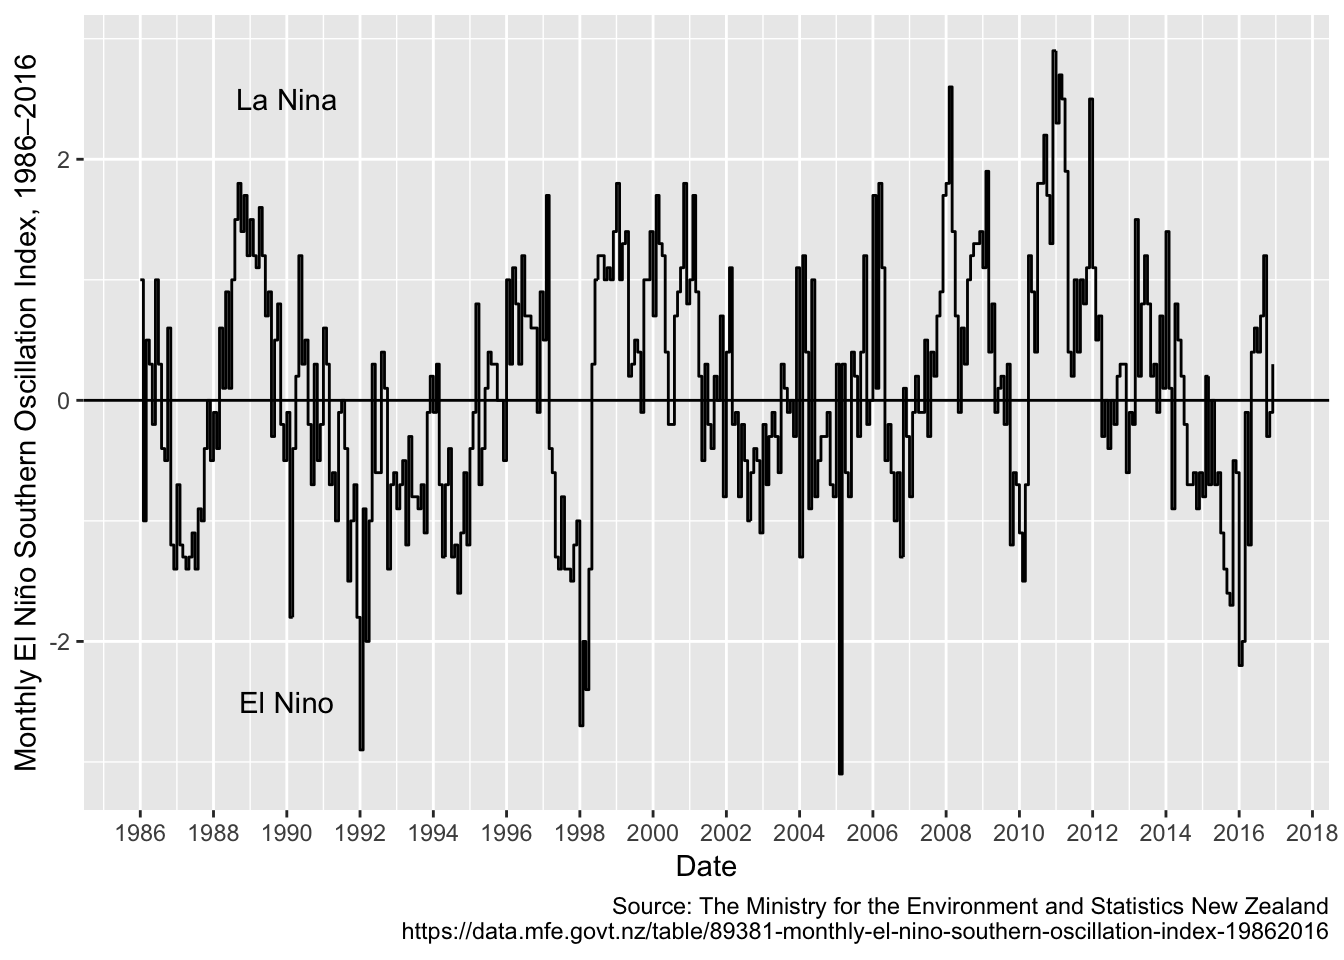
\includegraphics{nzElecGenTrends_files/figure-latex/monthlySOI-1.pdf}
\caption{\label{fig:monthlySOI}Monthly Southern Oscillation}
\end{figure}

Figure \ref(fig:yearlySOI) confirms this overall pattern although the
aggregation to calendar years (as opposed to climate years) masks some
of the periods.

\begin{verbatim}
## Warning in grid.Call(C_stringMetric, as.graphicsAnnot(x$label)): font
## metrics unknown for Unicode character U+2013

## Warning in grid.Call(C_stringMetric, as.graphicsAnnot(x$label)): font
## metrics unknown for Unicode character U+2013
\end{verbatim}

\begin{verbatim}
## Warning in grid.Call(C_stringMetric, as.graphicsAnnot(x$label)): conversion
## failure on 'Mean monthly El Niño Southern Oscillation Index, 1986–2016' in
## 'mbcsToSbcs': dot substituted for <e2>
\end{verbatim}

\begin{verbatim}
## Warning in grid.Call(C_stringMetric, as.graphicsAnnot(x$label)): conversion
## failure on 'Mean monthly El Niño Southern Oscillation Index, 1986–2016' in
## 'mbcsToSbcs': dot substituted for <80>
\end{verbatim}

\begin{verbatim}
## Warning in grid.Call(C_stringMetric, as.graphicsAnnot(x$label)): conversion
## failure on 'Mean monthly El Niño Southern Oscillation Index, 1986–2016' in
## 'mbcsToSbcs': dot substituted for <93>
\end{verbatim}

\begin{verbatim}
## Warning in grid.Call(C_textBounds, as.graphicsAnnot(x$label), x$x, x$y, :
## conversion failure on 'Mean monthly El Niño Southern Oscillation Index,
## 1986–2016' in 'mbcsToSbcs': dot substituted for <e2>
\end{verbatim}

\begin{verbatim}
## Warning in grid.Call(C_textBounds, as.graphicsAnnot(x$label), x$x, x$y, :
## conversion failure on 'Mean monthly El Niño Southern Oscillation Index,
## 1986–2016' in 'mbcsToSbcs': dot substituted for <80>
\end{verbatim}

\begin{verbatim}
## Warning in grid.Call(C_textBounds, as.graphicsAnnot(x$label), x$x, x$y, :
## conversion failure on 'Mean monthly El Niño Southern Oscillation Index,
## 1986–2016' in 'mbcsToSbcs': dot substituted for <93>
\end{verbatim}

\begin{verbatim}
## Warning in grid.Call(C_textBounds, as.graphicsAnnot(x$label), x$x, x$y, :
## conversion failure on 'Mean monthly El Niño Southern Oscillation Index,
## 1986–2016' in 'mbcsToSbcs': dot substituted for <e2>
\end{verbatim}

\begin{verbatim}
## Warning in grid.Call(C_textBounds, as.graphicsAnnot(x$label), x$x, x$y, :
## conversion failure on 'Mean monthly El Niño Southern Oscillation Index,
## 1986–2016' in 'mbcsToSbcs': dot substituted for <80>
\end{verbatim}

\begin{verbatim}
## Warning in grid.Call(C_textBounds, as.graphicsAnnot(x$label), x$x, x$y, :
## conversion failure on 'Mean monthly El Niño Southern Oscillation Index,
## 1986–2016' in 'mbcsToSbcs': dot substituted for <93>
\end{verbatim}

\begin{verbatim}
## Warning in grid.Call(C_textBounds, as.graphicsAnnot(x$label), x$x, x$y, :
## conversion failure on 'Mean monthly El Niño Southern Oscillation Index,
## 1986–2016' in 'mbcsToSbcs': dot substituted for <e2>
\end{verbatim}

\begin{verbatim}
## Warning in grid.Call(C_textBounds, as.graphicsAnnot(x$label), x$x, x$y, :
## conversion failure on 'Mean monthly El Niño Southern Oscillation Index,
## 1986–2016' in 'mbcsToSbcs': dot substituted for <80>
\end{verbatim}

\begin{verbatim}
## Warning in grid.Call(C_textBounds, as.graphicsAnnot(x$label), x$x, x$y, :
## conversion failure on 'Mean monthly El Niño Southern Oscillation Index,
## 1986–2016' in 'mbcsToSbcs': dot substituted for <93>
\end{verbatim}

\begin{verbatim}
## Warning in grid.Call(C_textBounds, as.graphicsAnnot(x$label), x$x, x$y, :
## conversion failure on 'Mean monthly El Niño Southern Oscillation Index,
## 1986–2016' in 'mbcsToSbcs': dot substituted for <e2>
\end{verbatim}

\begin{verbatim}
## Warning in grid.Call(C_textBounds, as.graphicsAnnot(x$label), x$x, x$y, :
## conversion failure on 'Mean monthly El Niño Southern Oscillation Index,
## 1986–2016' in 'mbcsToSbcs': dot substituted for <80>
\end{verbatim}

\begin{verbatim}
## Warning in grid.Call(C_textBounds, as.graphicsAnnot(x$label), x$x, x$y, :
## conversion failure on 'Mean monthly El Niño Southern Oscillation Index,
## 1986–2016' in 'mbcsToSbcs': dot substituted for <93>
\end{verbatim}

\begin{verbatim}
## Warning in grid.Call(C_textBounds, as.graphicsAnnot(x$label), x$x, x$y, :
## conversion failure on 'Mean monthly El Niño Southern Oscillation Index,
## 1986–2016' in 'mbcsToSbcs': dot substituted for <e2>
\end{verbatim}

\begin{verbatim}
## Warning in grid.Call(C_textBounds, as.graphicsAnnot(x$label), x$x, x$y, :
## conversion failure on 'Mean monthly El Niño Southern Oscillation Index,
## 1986–2016' in 'mbcsToSbcs': dot substituted for <80>
\end{verbatim}

\begin{verbatim}
## Warning in grid.Call(C_textBounds, as.graphicsAnnot(x$label), x$x, x$y, :
## conversion failure on 'Mean monthly El Niño Southern Oscillation Index,
## 1986–2016' in 'mbcsToSbcs': dot substituted for <93>
\end{verbatim}

\begin{verbatim}
## Warning in grid.Call(C_textBounds, as.graphicsAnnot(x$label), x$x, x$y, :
## conversion failure on 'Mean monthly El Niño Southern Oscillation Index,
## 1986–2016' in 'mbcsToSbcs': dot substituted for <e2>
\end{verbatim}

\begin{verbatim}
## Warning in grid.Call(C_textBounds, as.graphicsAnnot(x$label), x$x, x$y, :
## conversion failure on 'Mean monthly El Niño Southern Oscillation Index,
## 1986–2016' in 'mbcsToSbcs': dot substituted for <80>
\end{verbatim}

\begin{verbatim}
## Warning in grid.Call(C_textBounds, as.graphicsAnnot(x$label), x$x, x$y, :
## conversion failure on 'Mean monthly El Niño Southern Oscillation Index,
## 1986–2016' in 'mbcsToSbcs': dot substituted for <93>
\end{verbatim}

\begin{verbatim}
## Warning in grid.Call(C_textBounds, as.graphicsAnnot(x$label), x$x, x$y, :
## conversion failure on 'Mean monthly El Niño Southern Oscillation Index,
## 1986–2016' in 'mbcsToSbcs': dot substituted for <e2>
\end{verbatim}

\begin{verbatim}
## Warning in grid.Call(C_textBounds, as.graphicsAnnot(x$label), x$x, x$y, :
## conversion failure on 'Mean monthly El Niño Southern Oscillation Index,
## 1986–2016' in 'mbcsToSbcs': dot substituted for <80>
\end{verbatim}

\begin{verbatim}
## Warning in grid.Call(C_textBounds, as.graphicsAnnot(x$label), x$x, x$y, :
## conversion failure on 'Mean monthly El Niño Southern Oscillation Index,
## 1986–2016' in 'mbcsToSbcs': dot substituted for <93>
\end{verbatim}

\begin{verbatim}
## Warning in grid.Call.graphics(C_text, as.graphicsAnnot(x$label), x$x,
## x$y, : conversion failure on 'Mean monthly El Niño Southern Oscillation
## Index, 1986–2016' in 'mbcsToSbcs': dot substituted for <e2>
\end{verbatim}

\begin{verbatim}
## Warning in grid.Call.graphics(C_text, as.graphicsAnnot(x$label), x$x,
## x$y, : conversion failure on 'Mean monthly El Niño Southern Oscillation
## Index, 1986–2016' in 'mbcsToSbcs': dot substituted for <80>
\end{verbatim}

\begin{verbatim}
## Warning in grid.Call.graphics(C_text, as.graphicsAnnot(x$label), x$x,
## x$y, : conversion failure on 'Mean monthly El Niño Southern Oscillation
## Index, 1986–2016' in 'mbcsToSbcs': dot substituted for <93>
\end{verbatim}

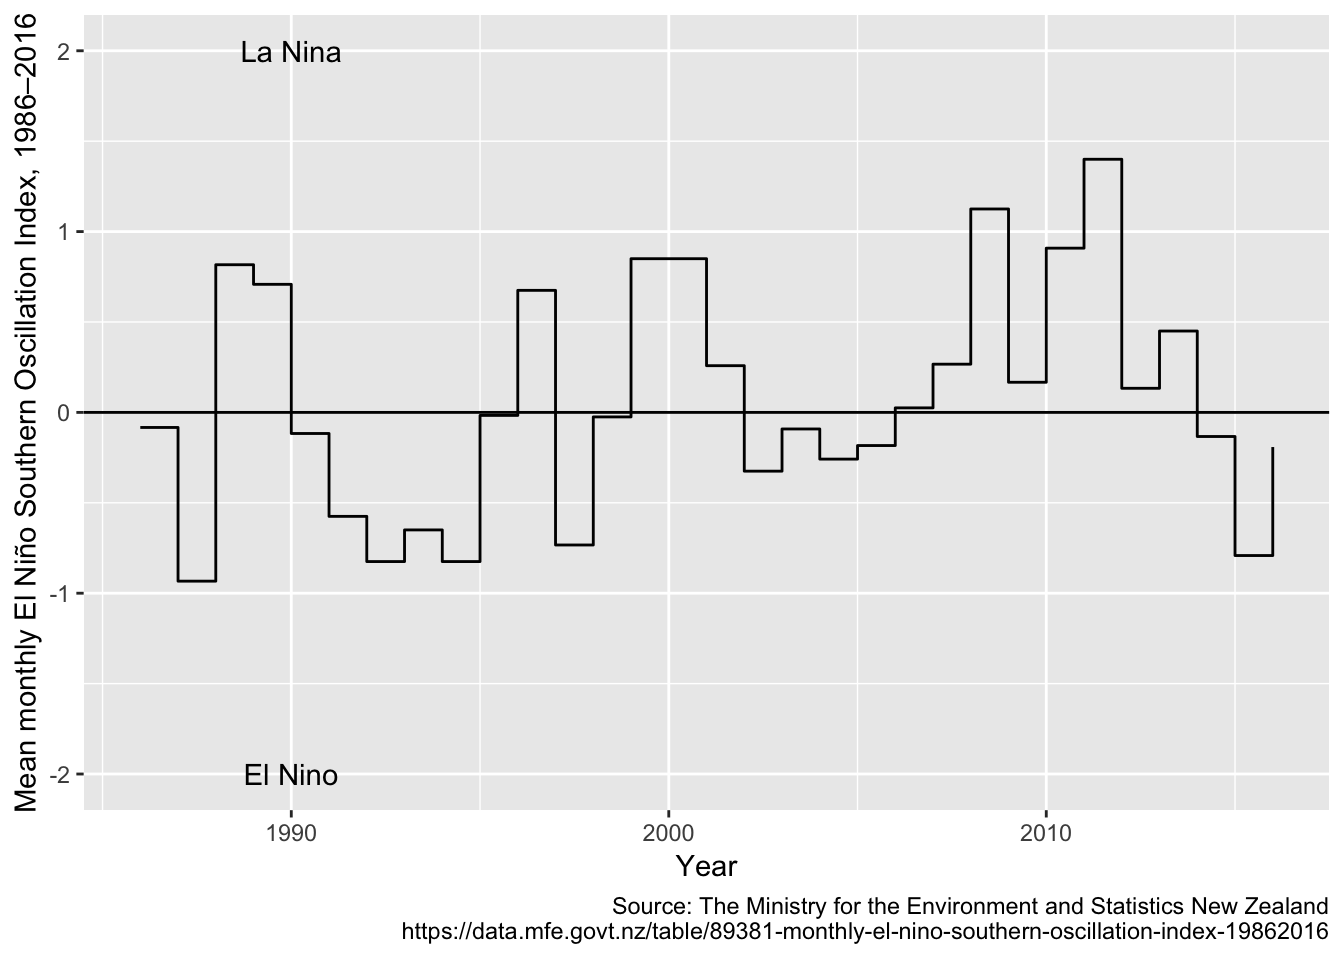
\includegraphics{nzElecGenTrends_files/figure-latex/yearlySOI-1.pdf}

\subsection{Yearly generation trends}\label{yearly-generation-trends}

Figure \ref{fig:yearlyTotalPlotPoint} shows the dominance of hydro and
decrease in coal use.

Adding annotations with information from:

\begin{itemize}
\tightlist
\item
  \url{https://www.niwa.co.nz/climate/summaries/seasonal}
\item
  \url{https://en.wikipedia.org/wiki/Huntly_Power_Station}
\end{itemize}

\begin{figure}
\centering
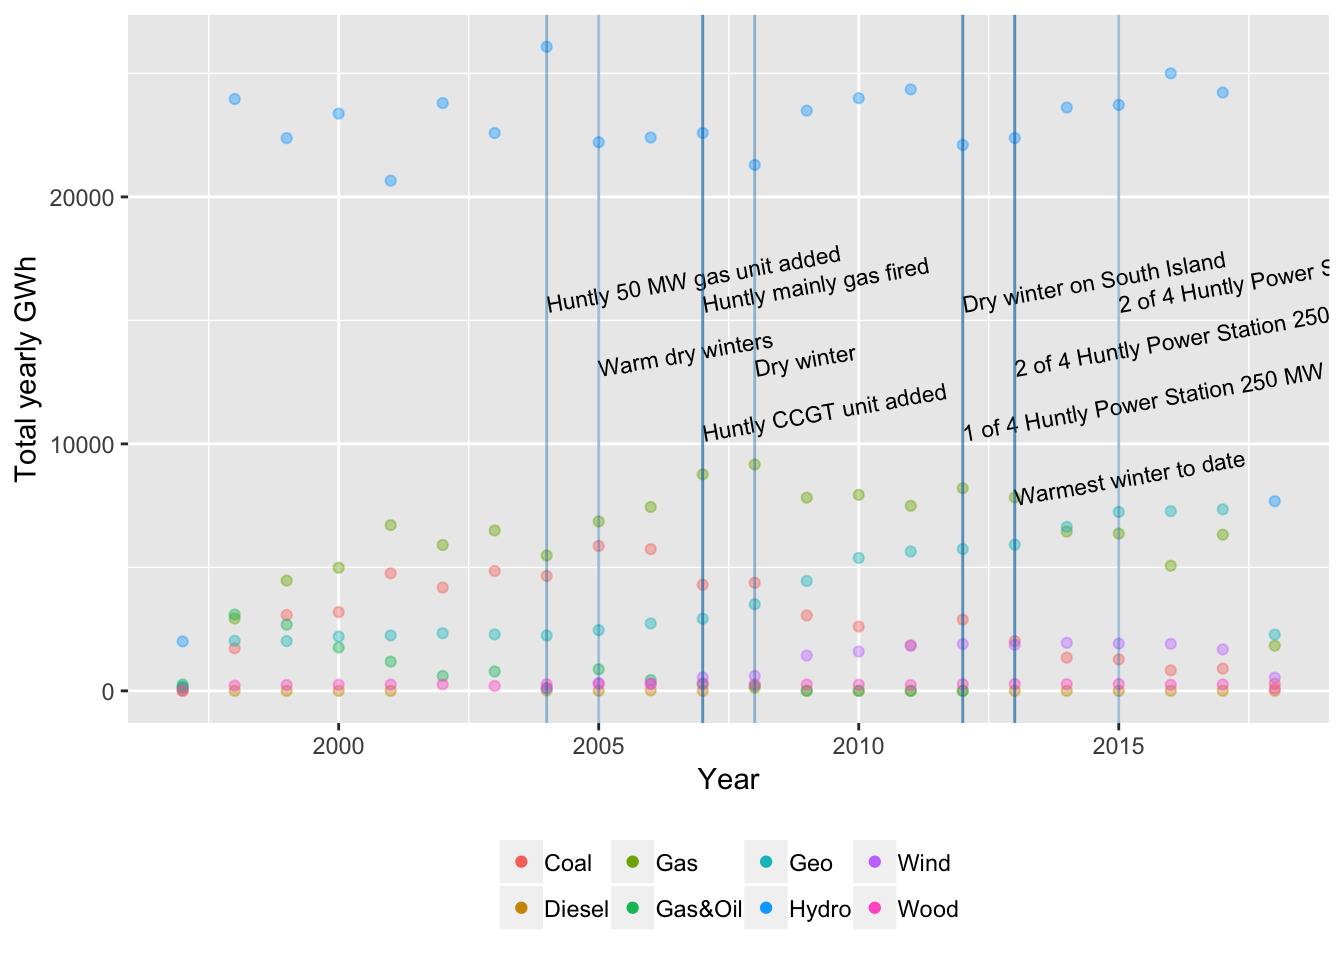
\includegraphics{nzElecGenTrends_files/figure-latex/yearlyTotalPlotPoint-1.pdf}
\caption{\label{fig:yearlyTotalPlotPoint}Yearly total plot by fuel type}
\end{figure}

If we consider the relationship between generation and the SOI at the
yearly level, Figure \ref(fig:yearlyGenSOI) suggests that Gas is fairly
responsive to increasing SOI above 0 (La Nina years) and hydro is the
inverse (with considerable variation/uncertainty) on an annual measure.
Presumably this indicates the use of Gas for peaking generation when
hydro is at capacity in drier years?

\begin{verbatim}
## Warning in grid.Call(C_stringMetric, as.graphicsAnnot(x$label)): font
## metrics unknown for Unicode character U+2013

## Warning in grid.Call(C_stringMetric, as.graphicsAnnot(x$label)): font
## metrics unknown for Unicode character U+2013
\end{verbatim}

\begin{verbatim}
## Warning in grid.Call(C_stringMetric, as.graphicsAnnot(x$label)): conversion
## failure on 'Monthly El Niño Southern Oscillation Index, 1986–2016' in
## 'mbcsToSbcs': dot substituted for <e2>
\end{verbatim}

\begin{verbatim}
## Warning in grid.Call(C_stringMetric, as.graphicsAnnot(x$label)): conversion
## failure on 'Monthly El Niño Southern Oscillation Index, 1986–2016' in
## 'mbcsToSbcs': dot substituted for <80>
\end{verbatim}

\begin{verbatim}
## Warning in grid.Call(C_stringMetric, as.graphicsAnnot(x$label)): conversion
## failure on 'Monthly El Niño Southern Oscillation Index, 1986–2016' in
## 'mbcsToSbcs': dot substituted for <93>
\end{verbatim}

\begin{verbatim}
## Warning in grid.Call(C_textBounds, as.graphicsAnnot(x$label), x$x, x$y, :
## conversion failure on 'Monthly El Niño Southern Oscillation Index, 1986–
## 2016' in 'mbcsToSbcs': dot substituted for <e2>
\end{verbatim}

\begin{verbatim}
## Warning in grid.Call(C_textBounds, as.graphicsAnnot(x$label), x$x, x$y, :
## conversion failure on 'Monthly El Niño Southern Oscillation Index, 1986–
## 2016' in 'mbcsToSbcs': dot substituted for <80>
\end{verbatim}

\begin{verbatim}
## Warning in grid.Call(C_textBounds, as.graphicsAnnot(x$label), x$x, x$y, :
## conversion failure on 'Monthly El Niño Southern Oscillation Index, 1986–
## 2016' in 'mbcsToSbcs': dot substituted for <93>
\end{verbatim}

\begin{verbatim}
## Warning in grid.Call(C_textBounds, as.graphicsAnnot(x$label), x$x, x$y, :
## conversion failure on 'Monthly El Niño Southern Oscillation Index, 1986–
## 2016' in 'mbcsToSbcs': dot substituted for <e2>
\end{verbatim}

\begin{verbatim}
## Warning in grid.Call(C_textBounds, as.graphicsAnnot(x$label), x$x, x$y, :
## conversion failure on 'Monthly El Niño Southern Oscillation Index, 1986–
## 2016' in 'mbcsToSbcs': dot substituted for <80>
\end{verbatim}

\begin{verbatim}
## Warning in grid.Call(C_textBounds, as.graphicsAnnot(x$label), x$x, x$y, :
## conversion failure on 'Monthly El Niño Southern Oscillation Index, 1986–
## 2016' in 'mbcsToSbcs': dot substituted for <93>
\end{verbatim}

\begin{verbatim}
## Warning in grid.Call(C_textBounds, as.graphicsAnnot(x$label), x$x, x$y, :
## conversion failure on 'Monthly El Niño Southern Oscillation Index, 1986–
## 2016' in 'mbcsToSbcs': dot substituted for <e2>
\end{verbatim}

\begin{verbatim}
## Warning in grid.Call(C_textBounds, as.graphicsAnnot(x$label), x$x, x$y, :
## conversion failure on 'Monthly El Niño Southern Oscillation Index, 1986–
## 2016' in 'mbcsToSbcs': dot substituted for <80>
\end{verbatim}

\begin{verbatim}
## Warning in grid.Call(C_textBounds, as.graphicsAnnot(x$label), x$x, x$y, :
## conversion failure on 'Monthly El Niño Southern Oscillation Index, 1986–
## 2016' in 'mbcsToSbcs': dot substituted for <93>
\end{verbatim}

\begin{verbatim}
## Warning in grid.Call(C_textBounds, as.graphicsAnnot(x$label), x$x, x$y, :
## conversion failure on 'Monthly El Niño Southern Oscillation Index, 1986–
## 2016' in 'mbcsToSbcs': dot substituted for <e2>
\end{verbatim}

\begin{verbatim}
## Warning in grid.Call(C_textBounds, as.graphicsAnnot(x$label), x$x, x$y, :
## conversion failure on 'Monthly El Niño Southern Oscillation Index, 1986–
## 2016' in 'mbcsToSbcs': dot substituted for <80>
\end{verbatim}

\begin{verbatim}
## Warning in grid.Call(C_textBounds, as.graphicsAnnot(x$label), x$x, x$y, :
## conversion failure on 'Monthly El Niño Southern Oscillation Index, 1986–
## 2016' in 'mbcsToSbcs': dot substituted for <93>
\end{verbatim}

\begin{verbatim}
## Warning in grid.Call(C_textBounds, as.graphicsAnnot(x$label), x$x, x$y, :
## conversion failure on 'Monthly El Niño Southern Oscillation Index, 1986–
## 2016' in 'mbcsToSbcs': dot substituted for <e2>
\end{verbatim}

\begin{verbatim}
## Warning in grid.Call(C_textBounds, as.graphicsAnnot(x$label), x$x, x$y, :
## conversion failure on 'Monthly El Niño Southern Oscillation Index, 1986–
## 2016' in 'mbcsToSbcs': dot substituted for <80>
\end{verbatim}

\begin{verbatim}
## Warning in grid.Call(C_textBounds, as.graphicsAnnot(x$label), x$x, x$y, :
## conversion failure on 'Monthly El Niño Southern Oscillation Index, 1986–
## 2016' in 'mbcsToSbcs': dot substituted for <93>
\end{verbatim}

\begin{verbatim}
## Warning in grid.Call(C_textBounds, as.graphicsAnnot(x$label), x$x, x$y, :
## conversion failure on 'Monthly El Niño Southern Oscillation Index, 1986–
## 2016' in 'mbcsToSbcs': dot substituted for <e2>
\end{verbatim}

\begin{verbatim}
## Warning in grid.Call(C_textBounds, as.graphicsAnnot(x$label), x$x, x$y, :
## conversion failure on 'Monthly El Niño Southern Oscillation Index, 1986–
## 2016' in 'mbcsToSbcs': dot substituted for <80>
\end{verbatim}

\begin{verbatim}
## Warning in grid.Call(C_textBounds, as.graphicsAnnot(x$label), x$x, x$y, :
## conversion failure on 'Monthly El Niño Southern Oscillation Index, 1986–
## 2016' in 'mbcsToSbcs': dot substituted for <93>
\end{verbatim}

\begin{verbatim}
## Warning in grid.Call(C_textBounds, as.graphicsAnnot(x$label), x$x, x$y, :
## conversion failure on 'Monthly El Niño Southern Oscillation Index, 1986–
## 2016' in 'mbcsToSbcs': dot substituted for <e2>
\end{verbatim}

\begin{verbatim}
## Warning in grid.Call(C_textBounds, as.graphicsAnnot(x$label), x$x, x$y, :
## conversion failure on 'Monthly El Niño Southern Oscillation Index, 1986–
## 2016' in 'mbcsToSbcs': dot substituted for <80>
\end{verbatim}

\begin{verbatim}
## Warning in grid.Call(C_textBounds, as.graphicsAnnot(x$label), x$x, x$y, :
## conversion failure on 'Monthly El Niño Southern Oscillation Index, 1986–
## 2016' in 'mbcsToSbcs': dot substituted for <93>
\end{verbatim}

\begin{verbatim}
## Warning in grid.Call.graphics(C_text, as.graphicsAnnot(x$label), x$x,
## x$y, : conversion failure on 'Monthly El Niño Southern Oscillation Index,
## 1986–2016' in 'mbcsToSbcs': dot substituted for <e2>
\end{verbatim}

\begin{verbatim}
## Warning in grid.Call.graphics(C_text, as.graphicsAnnot(x$label), x$x,
## x$y, : conversion failure on 'Monthly El Niño Southern Oscillation Index,
## 1986–2016' in 'mbcsToSbcs': dot substituted for <80>
\end{verbatim}

\begin{verbatim}
## Warning in grid.Call.graphics(C_text, as.graphicsAnnot(x$label), x$x,
## x$y, : conversion failure on 'Monthly El Niño Southern Oscillation Index,
## 1986–2016' in 'mbcsToSbcs': dot substituted for <93>
\end{verbatim}

\begin{figure}
\centering
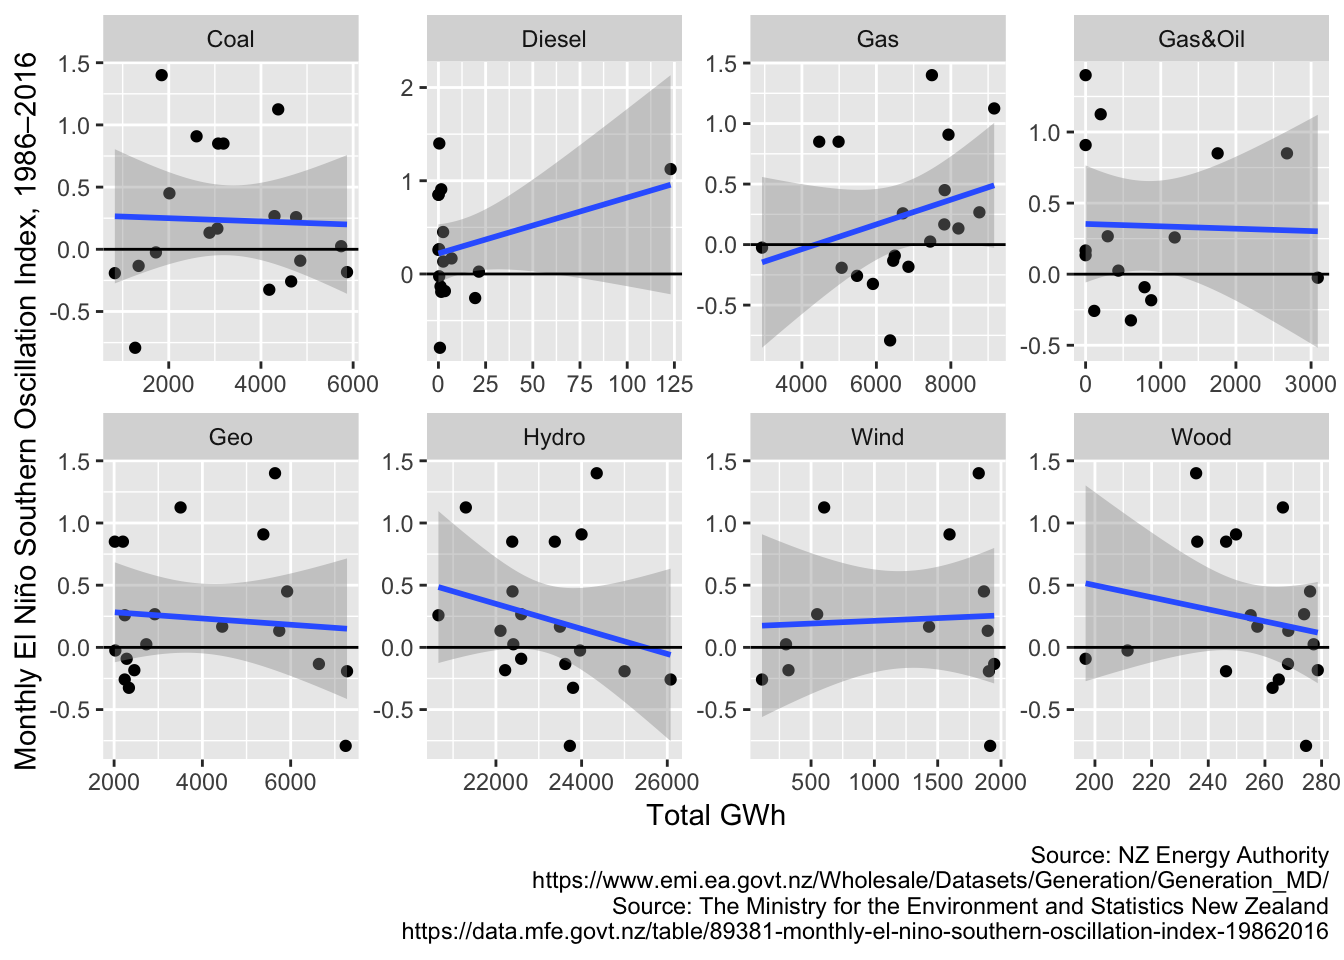
\includegraphics{nzElecGenTrends_files/figure-latex/yearlyGenSOI-1.pdf}
\caption{\label{fig:yearlyGenSOI}Yearly generation values by fuel vs yearly
SOI}
\end{figure}

\subsection{Monthly trends}\label{monthly-trends}

This section uses monthly aggregates.

\begin{verbatim}
## Warning: Removed 7 rows containing missing values (geom_path).
\end{verbatim}

\begin{figure}
\centering
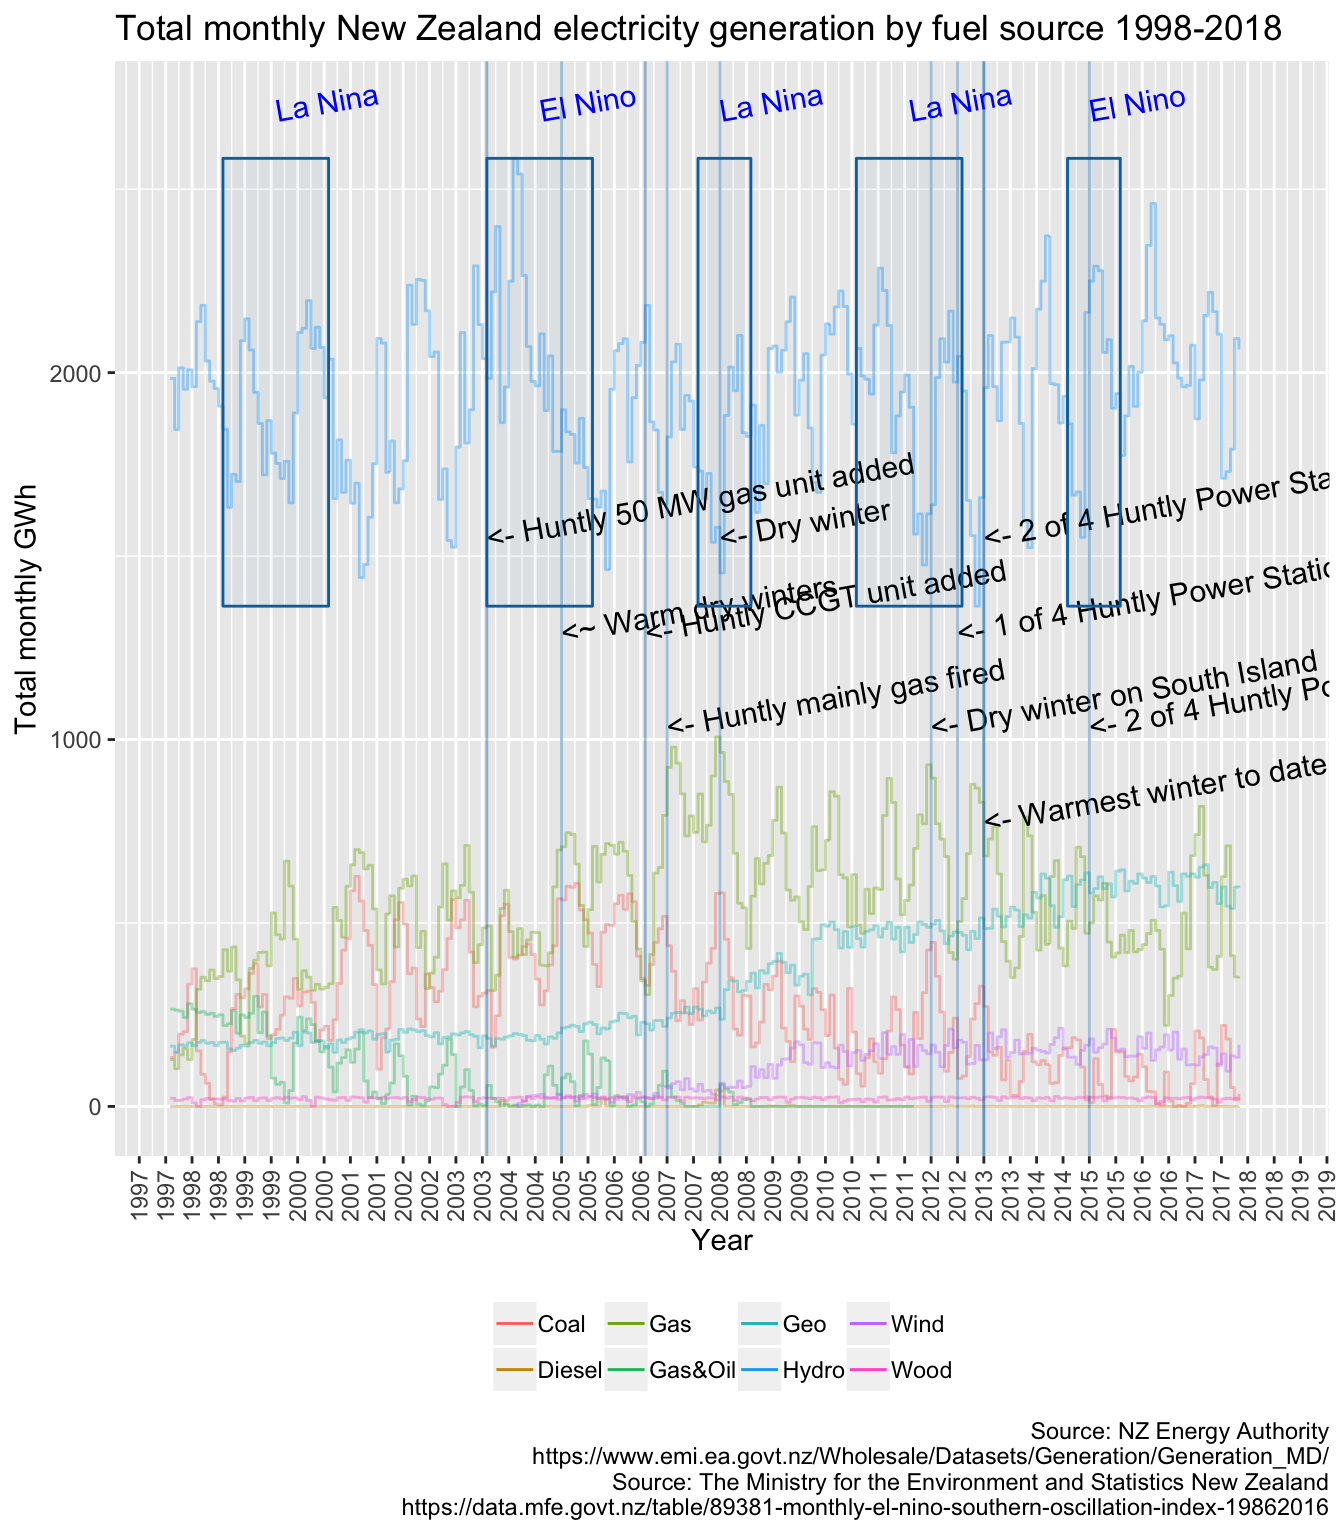
\includegraphics{nzElecGenTrends_files/figure-latex/monthlyTotalPlotPoint-1.pdf}
\caption{\label{fig:monthlyTotalPlotPoint}Yearly total plot by fuel type}
\end{figure}

\begin{verbatim}
## Saving 11 x 8 in image
\end{verbatim}

\begin{verbatim}
## Warning: Removed 7 rows containing missing values (geom_path).
\end{verbatim}

Figures \ref{fig:monthlyTotalPlotPoint} shows the same trends as
previously but using monthly data to highlight seasonal patterns over
time.

If we consider the relationship between generation and the SOI at the
monthly level, Figure \ref(fig:monthlyGenSOI) suggests there is a much
less clear relationship although the fit lines are still in the same
directions with increased use of gas as the SOI increases and the
inverse for hydro.

\begin{verbatim}
## Warning in grid.Call(C_stringMetric, as.graphicsAnnot(x$label)): font
## metrics unknown for Unicode character U+2013

## Warning in grid.Call(C_stringMetric, as.graphicsAnnot(x$label)): font
## metrics unknown for Unicode character U+2013
\end{verbatim}

\begin{verbatim}
## Warning in grid.Call(C_stringMetric, as.graphicsAnnot(x$label)): conversion
## failure on 'Monthly El Niño Southern Oscillation Index, 1986–2016' in
## 'mbcsToSbcs': dot substituted for <e2>
\end{verbatim}

\begin{verbatim}
## Warning in grid.Call(C_stringMetric, as.graphicsAnnot(x$label)): conversion
## failure on 'Monthly El Niño Southern Oscillation Index, 1986–2016' in
## 'mbcsToSbcs': dot substituted for <80>
\end{verbatim}

\begin{verbatim}
## Warning in grid.Call(C_stringMetric, as.graphicsAnnot(x$label)): conversion
## failure on 'Monthly El Niño Southern Oscillation Index, 1986–2016' in
## 'mbcsToSbcs': dot substituted for <93>
\end{verbatim}

\begin{verbatim}
## Warning in grid.Call(C_textBounds, as.graphicsAnnot(x$label), x$x, x$y, :
## conversion failure on 'Monthly El Niño Southern Oscillation Index, 1986–
## 2016' in 'mbcsToSbcs': dot substituted for <e2>
\end{verbatim}

\begin{verbatim}
## Warning in grid.Call(C_textBounds, as.graphicsAnnot(x$label), x$x, x$y, :
## conversion failure on 'Monthly El Niño Southern Oscillation Index, 1986–
## 2016' in 'mbcsToSbcs': dot substituted for <80>
\end{verbatim}

\begin{verbatim}
## Warning in grid.Call(C_textBounds, as.graphicsAnnot(x$label), x$x, x$y, :
## conversion failure on 'Monthly El Niño Southern Oscillation Index, 1986–
## 2016' in 'mbcsToSbcs': dot substituted for <93>
\end{verbatim}

\begin{verbatim}
## Warning in grid.Call(C_textBounds, as.graphicsAnnot(x$label), x$x, x$y, :
## conversion failure on 'Monthly El Niño Southern Oscillation Index, 1986–
## 2016' in 'mbcsToSbcs': dot substituted for <e2>
\end{verbatim}

\begin{verbatim}
## Warning in grid.Call(C_textBounds, as.graphicsAnnot(x$label), x$x, x$y, :
## conversion failure on 'Monthly El Niño Southern Oscillation Index, 1986–
## 2016' in 'mbcsToSbcs': dot substituted for <80>
\end{verbatim}

\begin{verbatim}
## Warning in grid.Call(C_textBounds, as.graphicsAnnot(x$label), x$x, x$y, :
## conversion failure on 'Monthly El Niño Southern Oscillation Index, 1986–
## 2016' in 'mbcsToSbcs': dot substituted for <93>
\end{verbatim}

\begin{verbatim}
## Warning in grid.Call(C_textBounds, as.graphicsAnnot(x$label), x$x, x$y, :
## conversion failure on 'Monthly El Niño Southern Oscillation Index, 1986–
## 2016' in 'mbcsToSbcs': dot substituted for <e2>
\end{verbatim}

\begin{verbatim}
## Warning in grid.Call(C_textBounds, as.graphicsAnnot(x$label), x$x, x$y, :
## conversion failure on 'Monthly El Niño Southern Oscillation Index, 1986–
## 2016' in 'mbcsToSbcs': dot substituted for <80>
\end{verbatim}

\begin{verbatim}
## Warning in grid.Call(C_textBounds, as.graphicsAnnot(x$label), x$x, x$y, :
## conversion failure on 'Monthly El Niño Southern Oscillation Index, 1986–
## 2016' in 'mbcsToSbcs': dot substituted for <93>
\end{verbatim}

\begin{verbatim}
## Warning in grid.Call(C_textBounds, as.graphicsAnnot(x$label), x$x, x$y, :
## conversion failure on 'Monthly El Niño Southern Oscillation Index, 1986–
## 2016' in 'mbcsToSbcs': dot substituted for <e2>
\end{verbatim}

\begin{verbatim}
## Warning in grid.Call(C_textBounds, as.graphicsAnnot(x$label), x$x, x$y, :
## conversion failure on 'Monthly El Niño Southern Oscillation Index, 1986–
## 2016' in 'mbcsToSbcs': dot substituted for <80>
\end{verbatim}

\begin{verbatim}
## Warning in grid.Call(C_textBounds, as.graphicsAnnot(x$label), x$x, x$y, :
## conversion failure on 'Monthly El Niño Southern Oscillation Index, 1986–
## 2016' in 'mbcsToSbcs': dot substituted for <93>
\end{verbatim}

\begin{verbatim}
## Warning in grid.Call(C_textBounds, as.graphicsAnnot(x$label), x$x, x$y, :
## conversion failure on 'Monthly El Niño Southern Oscillation Index, 1986–
## 2016' in 'mbcsToSbcs': dot substituted for <e2>
\end{verbatim}

\begin{verbatim}
## Warning in grid.Call(C_textBounds, as.graphicsAnnot(x$label), x$x, x$y, :
## conversion failure on 'Monthly El Niño Southern Oscillation Index, 1986–
## 2016' in 'mbcsToSbcs': dot substituted for <80>
\end{verbatim}

\begin{verbatim}
## Warning in grid.Call(C_textBounds, as.graphicsAnnot(x$label), x$x, x$y, :
## conversion failure on 'Monthly El Niño Southern Oscillation Index, 1986–
## 2016' in 'mbcsToSbcs': dot substituted for <93>
\end{verbatim}

\begin{verbatim}
## Warning in grid.Call(C_textBounds, as.graphicsAnnot(x$label), x$x, x$y, :
## conversion failure on 'Monthly El Niño Southern Oscillation Index, 1986–
## 2016' in 'mbcsToSbcs': dot substituted for <e2>
\end{verbatim}

\begin{verbatim}
## Warning in grid.Call(C_textBounds, as.graphicsAnnot(x$label), x$x, x$y, :
## conversion failure on 'Monthly El Niño Southern Oscillation Index, 1986–
## 2016' in 'mbcsToSbcs': dot substituted for <80>
\end{verbatim}

\begin{verbatim}
## Warning in grid.Call(C_textBounds, as.graphicsAnnot(x$label), x$x, x$y, :
## conversion failure on 'Monthly El Niño Southern Oscillation Index, 1986–
## 2016' in 'mbcsToSbcs': dot substituted for <93>
\end{verbatim}

\begin{verbatim}
## Warning in grid.Call(C_textBounds, as.graphicsAnnot(x$label), x$x, x$y, :
## conversion failure on 'Monthly El Niño Southern Oscillation Index, 1986–
## 2016' in 'mbcsToSbcs': dot substituted for <e2>
\end{verbatim}

\begin{verbatim}
## Warning in grid.Call(C_textBounds, as.graphicsAnnot(x$label), x$x, x$y, :
## conversion failure on 'Monthly El Niño Southern Oscillation Index, 1986–
## 2016' in 'mbcsToSbcs': dot substituted for <80>
\end{verbatim}

\begin{verbatim}
## Warning in grid.Call(C_textBounds, as.graphicsAnnot(x$label), x$x, x$y, :
## conversion failure on 'Monthly El Niño Southern Oscillation Index, 1986–
## 2016' in 'mbcsToSbcs': dot substituted for <93>
\end{verbatim}

\begin{verbatim}
## Warning in grid.Call.graphics(C_text, as.graphicsAnnot(x$label), x$x,
## x$y, : conversion failure on 'Monthly El Niño Southern Oscillation Index,
## 1986–2016' in 'mbcsToSbcs': dot substituted for <e2>
\end{verbatim}

\begin{verbatim}
## Warning in grid.Call.graphics(C_text, as.graphicsAnnot(x$label), x$x,
## x$y, : conversion failure on 'Monthly El Niño Southern Oscillation Index,
## 1986–2016' in 'mbcsToSbcs': dot substituted for <80>
\end{verbatim}

\begin{verbatim}
## Warning in grid.Call.graphics(C_text, as.graphicsAnnot(x$label), x$x,
## x$y, : conversion failure on 'Monthly El Niño Southern Oscillation Index,
## 1986–2016' in 'mbcsToSbcs': dot substituted for <93>
\end{verbatim}

\begin{figure}
\centering
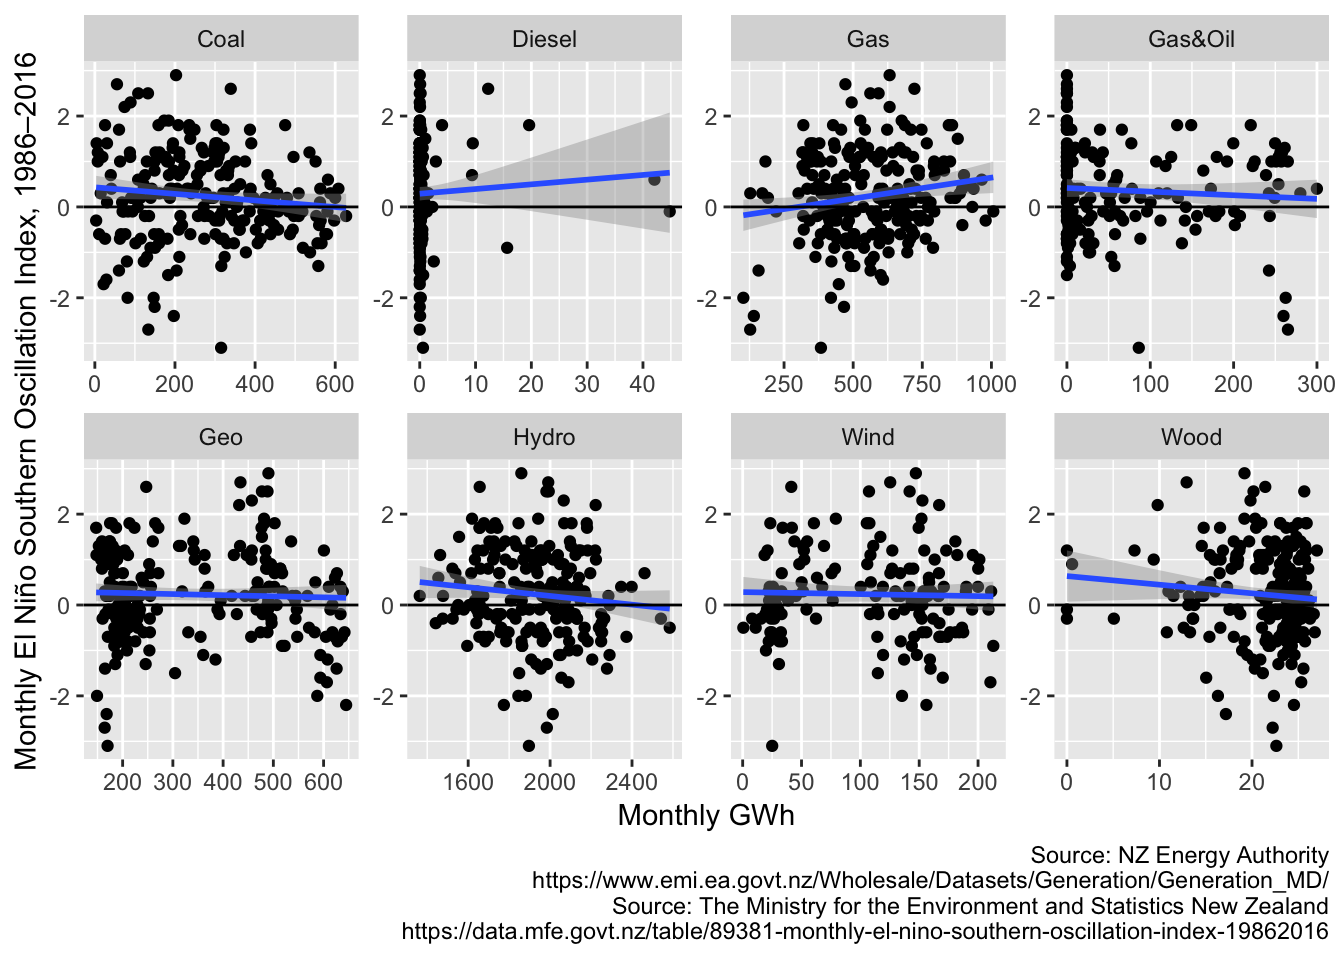
\includegraphics{nzElecGenTrends_files/figure-latex/monthlyGenSOI-1.pdf}
\caption{\label{fig:monthlyGenSOI}Yearly generation values by fuel vs yearly
SOI}
\end{figure}

\subsection{Daily trends}\label{daily-trends}

Figures \ref{fig:dailyTotalPlotPoint} and \ref{fig:dailyTotalPlotCol}
show the same trends as previously but using daily data to highlight
seasonal patterns over time. Annotations use information from:

\begin{itemize}
\tightlist
\item
  \url{https://www.niwa.co.nz/climate/summaries/seasonal}
\item
  \url{https://en.wikipedia.org/wiki/Huntly_Power_Station}
\end{itemize}

\begin{verbatim}
## Warning: Removed 217 rows containing missing values (geom_path).
\end{verbatim}

\begin{figure}
\centering
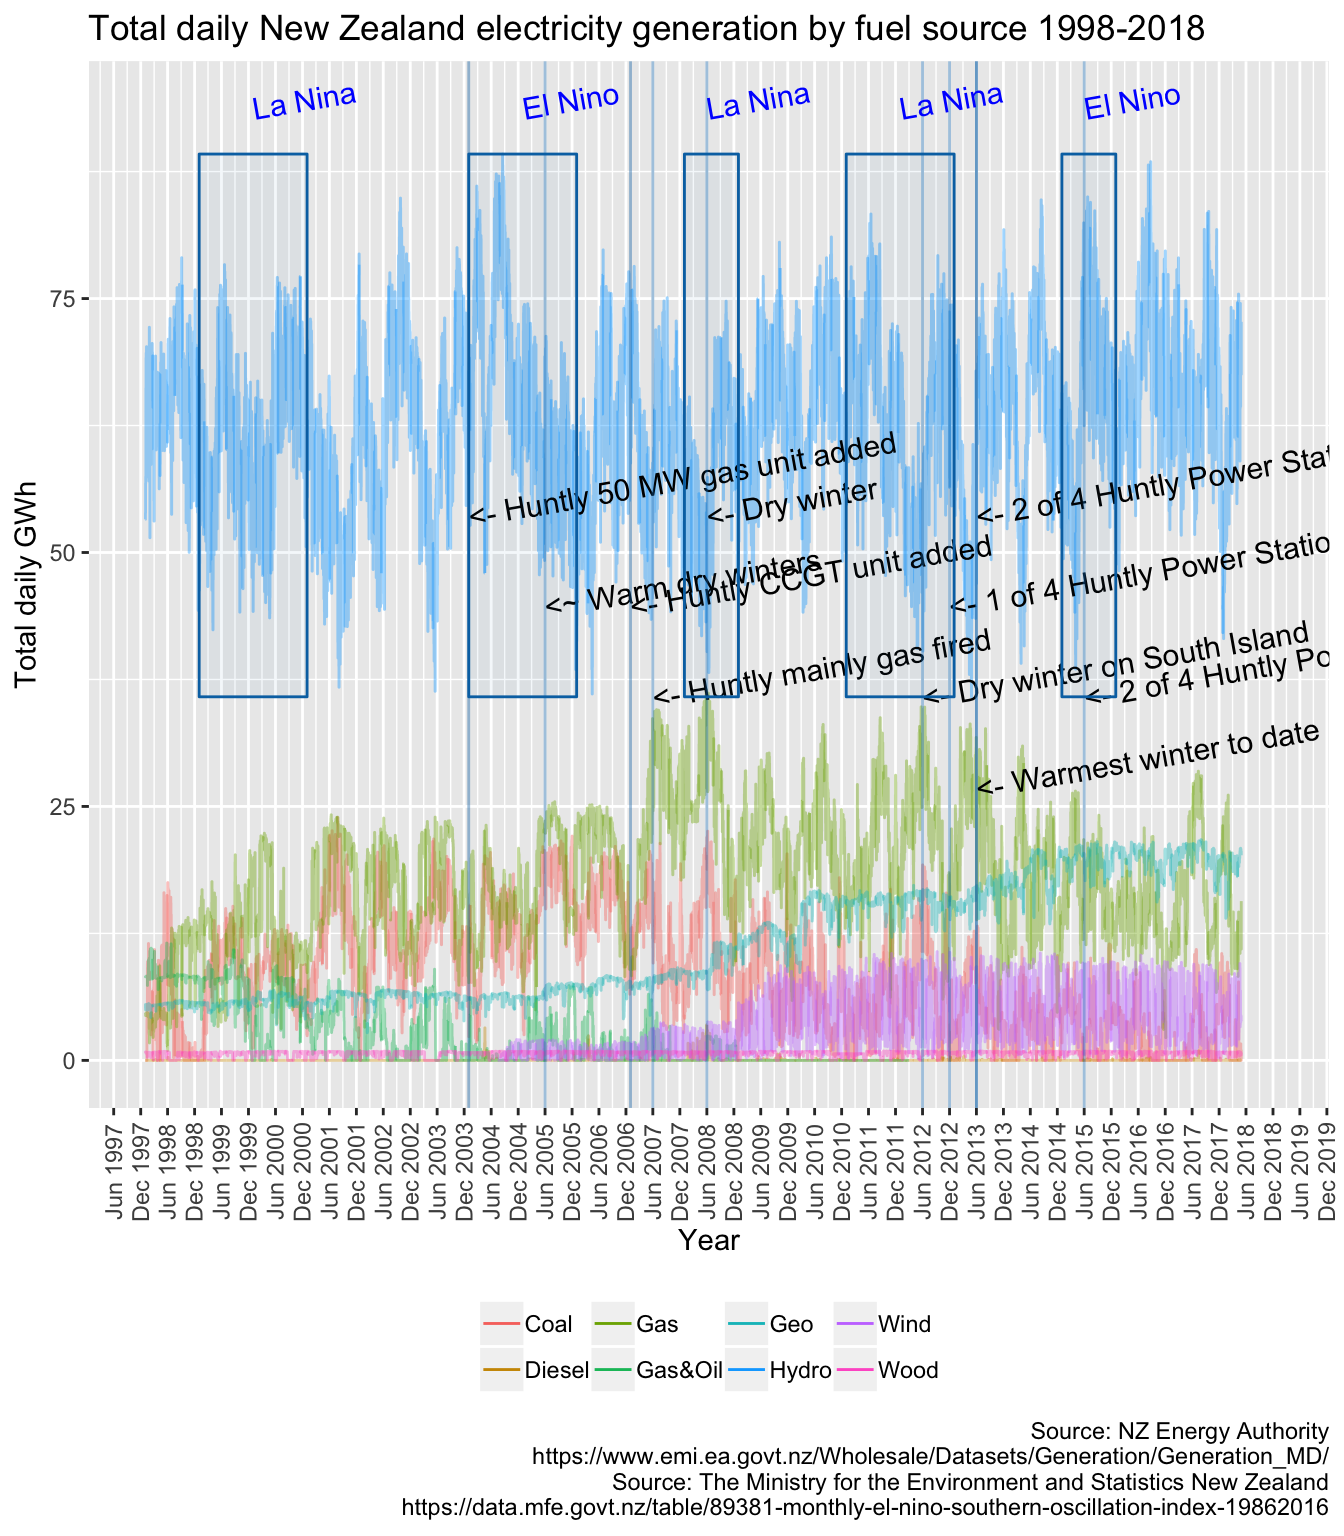
\includegraphics{nzElecGenTrends_files/figure-latex/dailyTotalPlotPoint-1.pdf}
\caption{\label{fig:dailyTotalPlotPoint}Yearly total plot by fuel type}
\end{figure}

\begin{verbatim}
## Saving 11 x 8 in image
\end{verbatim}

\begin{verbatim}
## Warning: Removed 217 rows containing missing values (geom_path).
\end{verbatim}

\section{Discussion}\label{discussion}

here

\section{Conclusions}\label{conclusions}

go here

\subsection{Data issues}\label{data-issues}

\subsubsection{Huntly 1-4 Fuel source}\label{huntly-1-4-fuel-source}

Figure \ref{fig:checkHuntly} shows the fuel use by each of the Huntly
units over time. It appears to show that huntly\_1\_4 always burns coal
although the units are able to also burn gas. It is not clear if this
data is correct.

\begin{figure}
\centering
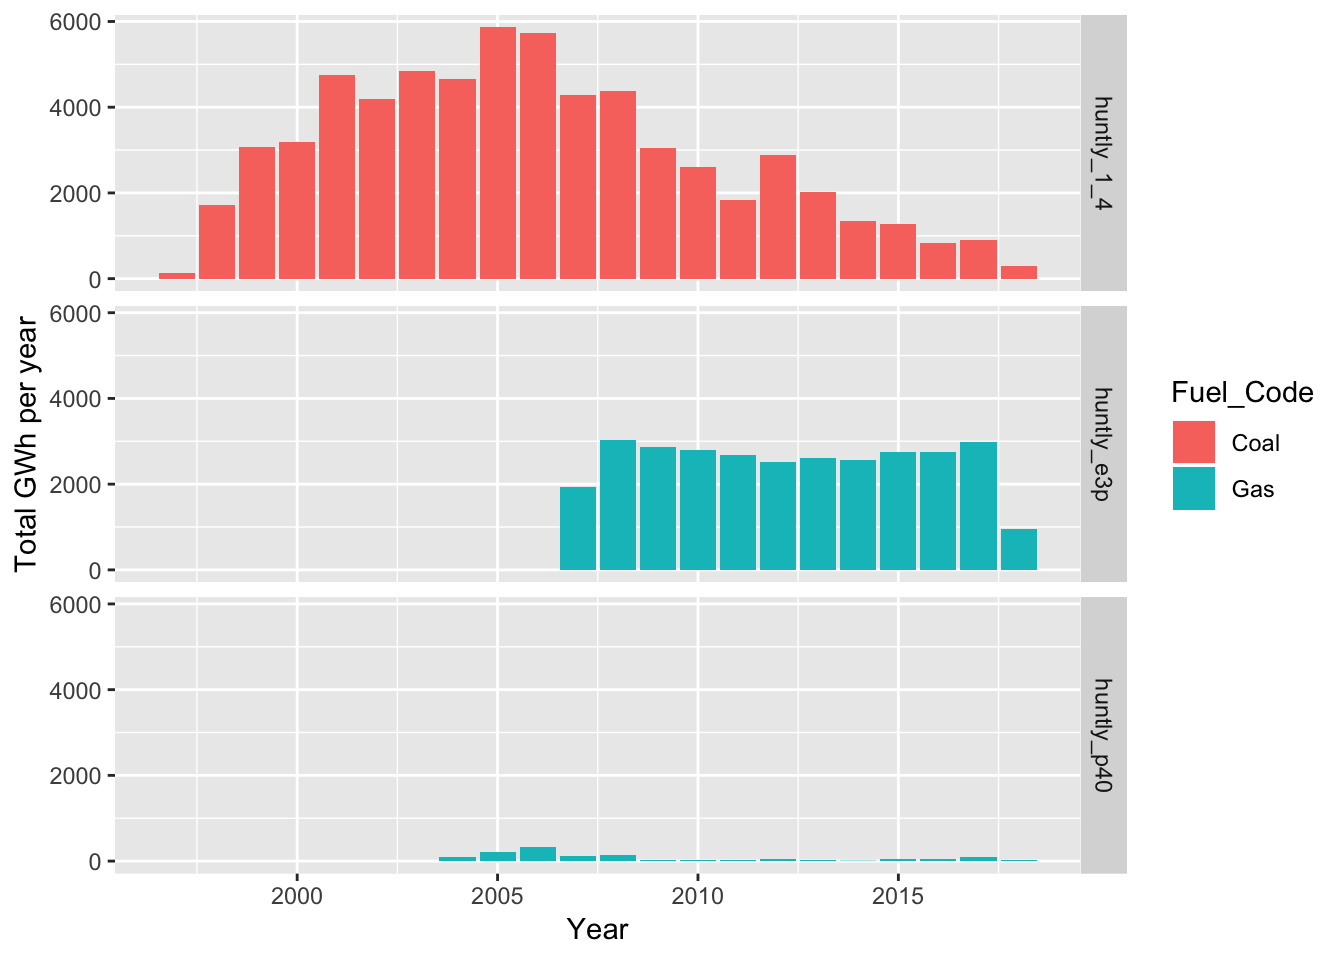
\includegraphics{nzElecGenTrends_files/figure-latex/checkHuntly-1.pdf}
\caption{\label{fig:checkHuntly}Huntly fuel sources}
\end{figure}

\subsubsection{What to do about TP49 \&
TP50?}\label{what-to-do-about-tp49-tp50}

\subsubsection{Solar \& embedded
generation}\label{solar-embedded-generation}

Should we be adding embedded generation from
\url{https://www.emi.ea.govt.nz/Wholesale/Datasets/Metered_data/Embedded_generation}
?

\section{Runtime}\label{runtime}

Analysis completed in 614.76 seconds ( 10.25 minutes) using
\href{https://cran.r-project.org/package=knitr}{knitr} in
\href{http://www.rstudio.com}{RStudio} with R version 3.5.0 (2018-04-23)
running on x86\_64-apple-darwin15.6.0.

\section{R environment}\label{r-environment}

R packages used:

\begin{itemize}
\tightlist
\item
  base R - for the basics (R Core Team 2016)
\item
  data.table - for fast (big) data handling (Dowle et al. 2015)
\item
  lubridate - date manipulation (Grolemund and Wickham 2011)
\item
  ggplot2 - for slick graphics (Wickham 2009)
\item
  readr - for csv reading/writing (Wickham, Hester, and Francois 2016)
\item
  Hmisc - for describe (Harrell Jr, Charles Dupont, and others. 2016)
\item
  knitr - to create this document \& neat tables (Xie 2016b)
\item
  bookdown - for additional markdown (Xie 2016a)
\item
  nzGREENGrid - for local NZ GREEN Grid project utilities
\end{itemize}

Session info:

\begin{verbatim}
## R version 3.5.0 (2018-04-23)
## Platform: x86_64-apple-darwin15.6.0 (64-bit)
## Running under: macOS High Sierra 10.13.5
## 
## Matrix products: default
## BLAS: /Library/Frameworks/R.framework/Versions/3.5/Resources/lib/libRblas.0.dylib
## LAPACK: /Library/Frameworks/R.framework/Versions/3.5/Resources/lib/libRlapack.dylib
## 
## locale:
## [1] en_GB.UTF-8/en_GB.UTF-8/en_GB.UTF-8/C/en_GB.UTF-8/en_GB.UTF-8
## 
## attached base packages:
## [1] stats     graphics  grDevices utils     datasets  methods   base     
## 
## other attached packages:
##  [1] knitr_1.20        Hmisc_4.1-1       Formula_1.2-3    
##  [4] survival_2.42-3   lattice_0.20-35   skimr_1.0.3      
##  [7] readr_1.1.1       ggplot2_2.2.1     dplyr_0.7.5      
## [10] data.table_1.11.4 nzGREENGrid_0.1.0
## 
## loaded via a namespace (and not attached):
##  [1] Rcpp_0.12.17        lubridate_1.7.4     prettyunits_1.0.2  
##  [4] png_0.1-7           utf8_1.1.4          assertthat_0.2.0   
##  [7] rprojroot_1.3-2     digest_0.6.15       R6_2.2.2           
## [10] plyr_1.8.4          backports_1.1.2     acepack_1.4.1      
## [13] evaluate_0.10.1     highr_0.7           pillar_1.2.3       
## [16] RgoogleMaps_1.4.2   rlang_0.2.1         progress_1.2.0     
## [19] lazyeval_0.2.1      rstudioapi_0.7      geosphere_1.5-7    
## [22] rpart_4.1-13        Matrix_1.2-14       checkmate_1.8.5    
## [25] rmarkdown_1.10      labeling_0.3        proto_1.0.0        
## [28] splines_3.5.0       stringr_1.3.1       foreign_0.8-70     
## [31] htmlwidgets_1.2     munsell_0.5.0       compiler_3.5.0     
## [34] xfun_0.1            pkgconfig_2.0.1     base64enc_0.1-3    
## [37] htmltools_0.3.6     nnet_7.3-12         openssl_1.0.1      
## [40] tidyselect_0.2.4    tibble_1.4.2        gridExtra_2.3      
## [43] htmlTable_1.12      bookdown_0.7        crayon_1.3.4       
## [46] grid_3.5.0          gtable_0.2.0        magrittr_1.5       
## [49] scales_0.5.0        cli_1.0.0           stringi_1.2.3      
## [52] mapproj_1.2.6       reshape2_1.4.3      bindrcpp_0.2.2     
## [55] sp_1.3-1            latticeExtra_0.6-28 rjson_0.2.20       
## [58] RColorBrewer_1.1-2  tools_3.5.0         ggmap_2.6.1        
## [61] glue_1.2.0          purrr_0.2.5         maps_3.3.0         
## [64] hms_0.4.2           jpeg_0.1-8          yaml_2.1.19        
## [67] colorspace_1.3-2    cluster_2.0.7-1     bindr_0.1.1
\end{verbatim}

\section*{References}\label{references}
\addcontentsline{toc}{section}{References}

\hypertarget{refs}{}
\hypertarget{ref-data.table}{}
Dowle, M, A Srinivasan, T Short, S Lianoglou with contributions from R
Saporta, and E Antonyan. 2015. \emph{Data.table: Extension of
Data.frame}. \url{https://CRAN.R-project.org/package=data.table}.

\hypertarget{ref-lubridate}{}
Grolemund, Garrett, and Hadley Wickham. 2011. ``Dates and Times Made
Easy with lubridate.'' \emph{Journal of Statistical Software} 40 (3):
1--25. \url{http://www.jstatsoft.org/v40/i03/}.

\hypertarget{ref-Hmisc}{}
Harrell Jr, Frank E, with contributions from Charles Dupont, and many
others. 2016. \emph{Hmisc: Harrell Miscellaneous}.
\url{https://CRAN.R-project.org/package=Hmisc}.

\hypertarget{ref-baseR}{}
R Core Team. 2016. \emph{R: A Language and Environment for Statistical
Computing}. Vienna, Austria: R Foundation for Statistical Computing.
\url{https://www.R-project.org/}.

\hypertarget{ref-ggplot2}{}
Wickham, Hadley. 2009. \emph{Ggplot2: Elegant Graphics for Data
Analysis}. Springer-Verlag New York. \url{http://ggplot2.org}.

\hypertarget{ref-readr}{}
Wickham, Hadley, Jim Hester, and Romain Francois. 2016. \emph{Readr:
Read Tabular Data}. \url{https://CRAN.R-project.org/package=readr}.

\hypertarget{ref-bookdown}{}
Xie, Yihui. 2016a. \emph{Bookdown: Authoring Books and Technical
Documents with R Markdown}. Boca Raton, Florida: Chapman; Hall/CRC.
\url{https://github.com/rstudio/bookdown}.

\hypertarget{ref-knitr}{}
---------. 2016b. \emph{Knitr: A General-Purpose Package for Dynamic
Report Generation in R}. \url{https://CRAN.R-project.org/package=knitr}.


\end{document}
